% Options for packages loaded elsewhere
\PassOptionsToPackage{unicode}{hyperref}
\PassOptionsToPackage{hyphens}{url}
%
\documentclass[
]{article}
\usepackage{amsmath,amssymb}
\usepackage{iftex}
\ifPDFTeX
  \usepackage[T1]{fontenc}
  \usepackage[utf8]{inputenc}
  \usepackage{textcomp} % provide euro and other symbols
\else % if luatex or xetex
  \usepackage{unicode-math} % this also loads fontspec
  \defaultfontfeatures{Scale=MatchLowercase}
  \defaultfontfeatures[\rmfamily]{Ligatures=TeX,Scale=1}
\fi
\usepackage{lmodern}
\ifPDFTeX\else
  % xetex/luatex font selection
\fi
% Use upquote if available, for straight quotes in verbatim environments
\IfFileExists{upquote.sty}{\usepackage{upquote}}{}
\IfFileExists{microtype.sty}{% use microtype if available
  \usepackage[]{microtype}
  \UseMicrotypeSet[protrusion]{basicmath} % disable protrusion for tt fonts
}{}
\makeatletter
\@ifundefined{KOMAClassName}{% if non-KOMA class
  \IfFileExists{parskip.sty}{%
    \usepackage{parskip}
  }{% else
    \setlength{\parindent}{0pt}
    \setlength{\parskip}{6pt plus 2pt minus 1pt}}
}{% if KOMA class
  \KOMAoptions{parskip=half}}
\makeatother
\usepackage{xcolor}
\usepackage[landscape,margin=0.75in,margin=1in]{geometry}
\usepackage{color}
\usepackage{fancyvrb}
\newcommand{\VerbBar}{|}
\newcommand{\VERB}{\Verb[commandchars=\\\{\}]}
\DefineVerbatimEnvironment{Highlighting}{Verbatim}{commandchars=\\\{\}}
% Add ',fontsize=\small' for more characters per line
\usepackage{framed}
\definecolor{shadecolor}{RGB}{248,248,248}
\newenvironment{Shaded}{\begin{snugshade}}{\end{snugshade}}
\newcommand{\AlertTok}[1]{\textcolor[rgb]{0.94,0.16,0.16}{#1}}
\newcommand{\AnnotationTok}[1]{\textcolor[rgb]{0.56,0.35,0.01}{\textbf{\textit{#1}}}}
\newcommand{\AttributeTok}[1]{\textcolor[rgb]{0.13,0.29,0.53}{#1}}
\newcommand{\BaseNTok}[1]{\textcolor[rgb]{0.00,0.00,0.81}{#1}}
\newcommand{\BuiltInTok}[1]{#1}
\newcommand{\CharTok}[1]{\textcolor[rgb]{0.31,0.60,0.02}{#1}}
\newcommand{\CommentTok}[1]{\textcolor[rgb]{0.56,0.35,0.01}{\textit{#1}}}
\newcommand{\CommentVarTok}[1]{\textcolor[rgb]{0.56,0.35,0.01}{\textbf{\textit{#1}}}}
\newcommand{\ConstantTok}[1]{\textcolor[rgb]{0.56,0.35,0.01}{#1}}
\newcommand{\ControlFlowTok}[1]{\textcolor[rgb]{0.13,0.29,0.53}{\textbf{#1}}}
\newcommand{\DataTypeTok}[1]{\textcolor[rgb]{0.13,0.29,0.53}{#1}}
\newcommand{\DecValTok}[1]{\textcolor[rgb]{0.00,0.00,0.81}{#1}}
\newcommand{\DocumentationTok}[1]{\textcolor[rgb]{0.56,0.35,0.01}{\textbf{\textit{#1}}}}
\newcommand{\ErrorTok}[1]{\textcolor[rgb]{0.64,0.00,0.00}{\textbf{#1}}}
\newcommand{\ExtensionTok}[1]{#1}
\newcommand{\FloatTok}[1]{\textcolor[rgb]{0.00,0.00,0.81}{#1}}
\newcommand{\FunctionTok}[1]{\textcolor[rgb]{0.13,0.29,0.53}{\textbf{#1}}}
\newcommand{\ImportTok}[1]{#1}
\newcommand{\InformationTok}[1]{\textcolor[rgb]{0.56,0.35,0.01}{\textbf{\textit{#1}}}}
\newcommand{\KeywordTok}[1]{\textcolor[rgb]{0.13,0.29,0.53}{\textbf{#1}}}
\newcommand{\NormalTok}[1]{#1}
\newcommand{\OperatorTok}[1]{\textcolor[rgb]{0.81,0.36,0.00}{\textbf{#1}}}
\newcommand{\OtherTok}[1]{\textcolor[rgb]{0.56,0.35,0.01}{#1}}
\newcommand{\PreprocessorTok}[1]{\textcolor[rgb]{0.56,0.35,0.01}{\textit{#1}}}
\newcommand{\RegionMarkerTok}[1]{#1}
\newcommand{\SpecialCharTok}[1]{\textcolor[rgb]{0.81,0.36,0.00}{\textbf{#1}}}
\newcommand{\SpecialStringTok}[1]{\textcolor[rgb]{0.31,0.60,0.02}{#1}}
\newcommand{\StringTok}[1]{\textcolor[rgb]{0.31,0.60,0.02}{#1}}
\newcommand{\VariableTok}[1]{\textcolor[rgb]{0.00,0.00,0.00}{#1}}
\newcommand{\VerbatimStringTok}[1]{\textcolor[rgb]{0.31,0.60,0.02}{#1}}
\newcommand{\WarningTok}[1]{\textcolor[rgb]{0.56,0.35,0.01}{\textbf{\textit{#1}}}}
\usepackage{longtable,booktabs,array}
\usepackage{calc} % for calculating minipage widths
% Correct order of tables after \paragraph or \subparagraph
\usepackage{etoolbox}
\makeatletter
\patchcmd\longtable{\par}{\if@noskipsec\mbox{}\fi\par}{}{}
\makeatother
% Allow footnotes in longtable head/foot
\IfFileExists{footnotehyper.sty}{\usepackage{footnotehyper}}{\usepackage{footnote}}
\makesavenoteenv{longtable}
\usepackage{graphicx}
\makeatletter
\newsavebox\pandoc@box
\newcommand*\pandocbounded[1]{% scales image to fit in text height/width
  \sbox\pandoc@box{#1}%
  \Gscale@div\@tempa{\textheight}{\dimexpr\ht\pandoc@box+\dp\pandoc@box\relax}%
  \Gscale@div\@tempb{\linewidth}{\wd\pandoc@box}%
  \ifdim\@tempb\p@<\@tempa\p@\let\@tempa\@tempb\fi% select the smaller of both
  \ifdim\@tempa\p@<\p@\scalebox{\@tempa}{\usebox\pandoc@box}%
  \else\usebox{\pandoc@box}%
  \fi%
}
% Set default figure placement to htbp
\def\fps@figure{htbp}
\makeatother
\setlength{\emergencystretch}{3em} % prevent overfull lines
\providecommand{\tightlist}{%
  \setlength{\itemsep}{0pt}\setlength{\parskip}{0pt}}
\setcounter{secnumdepth}{5}
\usepackage{xcolor}
\usepackage{lscape}
\usepackage{booktabs}
\usepackage{longtable}
\usepackage{array}
\usepackage{multirow}
\usepackage{wrapfig}
\usepackage{float}
\usepackage{colortbl}
\usepackage{pdflscape}
\usepackage{tabu}
\usepackage{threeparttable}
\usepackage{threeparttablex}
\usepackage[normalem]{ulem}
\usepackage{makecell}
\usepackage{xcolor}
\usepackage{bookmark}
\IfFileExists{xurl.sty}{\usepackage{xurl}}{} % add URL line breaks if available
\urlstyle{same}
\hypersetup{
  pdftitle={Exploratory Data Analysys},
  pdfauthor={Barrett Viator and Ray Chandonnet},
  hidelinks,
  pdfcreator={LaTeX via pandoc}}

\title{Exploratory Data Analysys}
\author{Barrett Viator and Ray Chandonnet}
\date{2025-07-26}

\begin{document}
\maketitle

\textcolor{blue}{This code uses static data as its starting point rather than running a lengthy API call.  For production, to access realtime current data, this would be replaced by a call to the API using the reticulate functions that call Python code in R}

\begin{Shaded}
\begin{Highlighting}[]
\NormalTok{RawData }\OtherTok{\textless{}{-}} \FunctionTok{readRDS}\NormalTok{(here}\SpecialCharTok{::}\FunctionTok{here}\NormalTok{(}\StringTok{"Data"}\NormalTok{,}\StringTok{"PreEDA\_DataFrame.rds"}\NormalTok{))}
\FunctionTok{names}\NormalTok{(RawData) }\OtherTok{\textless{}{-}} \FunctionTok{make.unique}\NormalTok{(}\FunctionTok{names}\NormalTok{(RawData), }\AttributeTok{sep =} \StringTok{"."}\NormalTok{)}
\NormalTok{FieldActions }\OtherTok{\textless{}{-}} \FunctionTok{read\_excel}\NormalTok{(here}\SpecialCharTok{::}\FunctionTok{here}\NormalTok{(}\StringTok{"Data"}\NormalTok{, }\StringTok{"FieldActions.xlsx"}\NormalTok{))}
\NormalTok{CleanedData }\OtherTok{\textless{}{-}}\NormalTok{ RawData }\CommentTok{\# make a copy to preserve original}
\NormalTok{IncomeData }\OtherTok{\textless{}{-}} \FunctionTok{read\_excel}\NormalTok{(here}\SpecialCharTok{::}\FunctionTok{here}\NormalTok{(}\StringTok{"Data"}\NormalTok{, }\StringTok{"Income Group Data.xlsx"}\NormalTok{)) }\CommentTok{\# Import income data}
\end{Highlighting}
\end{Shaded}

\begin{Shaded}
\begin{Highlighting}[]
\CommentTok{\# This code iterates through every field in the raw data, taking the cleanup action on}
\CommentTok{\# it that is specified in the FieldActions data frame.  The net result is that a bunch of}
\CommentTok{\# duplicated and/or unneeded fields are deleted, fields with uninterpretable (coded) column }
\CommentTok{\# names tied to their source are renamed to be descriptive, and the Year column is forced }
\CommentTok{\# to an integer}

\ControlFlowTok{for}\NormalTok{ (fieldcounter }\ControlFlowTok{in} \FunctionTok{names}\NormalTok{(CleanedData)) \{}
\NormalTok{  action\_row }\OtherTok{\textless{}{-}}\NormalTok{ FieldActions[FieldActions}\SpecialCharTok{$}\NormalTok{FieldName }\SpecialCharTok{==}\NormalTok{ fieldcounter, ]}
  \ControlFlowTok{if}\NormalTok{ (}\FunctionTok{nrow}\NormalTok{(action\_row) }\SpecialCharTok{==} \DecValTok{0}\NormalTok{) \{}
    \ControlFlowTok{next}  \CommentTok{\# No action specified for this field}
\NormalTok{  \}}
\NormalTok{  WhatToDo }\OtherTok{\textless{}{-}}\NormalTok{ action\_row}\SpecialCharTok{$}\NormalTok{Action}
  \ControlFlowTok{if}\NormalTok{ (WhatToDo }\SpecialCharTok{==} \StringTok{"Delete"}\NormalTok{) \{}
\NormalTok{    CleanedData[[fieldcounter]] }\OtherTok{\textless{}{-}} \ConstantTok{NULL}
    
\NormalTok{  \} }\ControlFlowTok{else} \ControlFlowTok{if}\NormalTok{ (WhatToDo }\SpecialCharTok{==} \StringTok{"Rename"}\NormalTok{) \{}
    \FunctionTok{names}\NormalTok{(CleanedData)[}\FunctionTok{names}\NormalTok{(CleanedData) }\SpecialCharTok{==}\NormalTok{ fieldcounter] }\OtherTok{\textless{}{-}}\NormalTok{ action\_row}\SpecialCharTok{$}\NormalTok{RenamedTo}
    
\NormalTok{  \} }\ControlFlowTok{else} \ControlFlowTok{if}\NormalTok{ (WhatToDo }\SpecialCharTok{==} \StringTok{"Make Integer"}\NormalTok{) \{}
\NormalTok{    CleanedData[[fieldcounter]] }\OtherTok{\textless{}{-}} \FunctionTok{as.integer}\NormalTok{(CleanedData[[fieldcounter]])}
\NormalTok{  \}}
\NormalTok{\}}
\CommentTok{\# Now, pull in the Income Group Data, and join it to the raw data by CountryCode}
\NormalTok{CleanedData }\OtherTok{\textless{}{-}} \FunctionTok{left\_join}\NormalTok{(CleanedData, IncomeData, }\AttributeTok{by =} \FunctionTok{c}\NormalTok{(}\StringTok{"CountryCode"} \OtherTok{=} \StringTok{"Country Code"}\NormalTok{))}

\CommentTok{\# Now for initial EDA purposes, I am only going to consider the two wellbeing indexes}
\CommentTok{\# which are tagged as my PrimaryResponse fields.  So I want to drop the other more granular}
\CommentTok{\# Response fields}

\CommentTok{\# Select field names to keep}
\CommentTok{\# First, all the renamed fields that weren\textquotesingle{}t dropped and aren\textquotesingle{}t a Response}
\NormalTok{PrimaryFields }\OtherTok{\textless{}{-}}\NormalTok{ FieldActions }\SpecialCharTok{\%\textgreater{}\%}
  \FunctionTok{filter}\NormalTok{(Type }\SpecialCharTok{\%in\%} \FunctionTok{c}\NormalTok{(}\StringTok{"PrimaryResponse"}\NormalTok{,}\StringTok{"Predictor"}\NormalTok{,}\StringTok{"Identifier"}\NormalTok{),}
         \FunctionTok{is.na}\NormalTok{(Action) }\SpecialCharTok{|}\NormalTok{ Action }\SpecialCharTok{!=} \StringTok{"Delete"}\NormalTok{) }\SpecialCharTok{\%\textgreater{}\%}
  \FunctionTok{pull}\NormalTok{(RenamedTo)}
\CommentTok{\# Now add the Income Group field (since that was joined from a different data set)}
\NormalTok{PrimaryFields }\OtherTok{\textless{}{-}} \FunctionTok{c}\NormalTok{(PrimaryFields, }\StringTok{"Income Group"}\NormalTok{)}
\CommentTok{\# Subset the cleaned dataset using that list of fields}
\NormalTok{FirstCutData }\OtherTok{\textless{}{-}}\NormalTok{ CleanedData }\SpecialCharTok{\%\textgreater{}\%}
  \FunctionTok{select}\NormalTok{(}\FunctionTok{all\_of}\NormalTok{(PrimaryFields))}
\FunctionTok{write\_xlsx}\NormalTok{(FirstCutData, }\AttributeTok{path =}\NormalTok{ here}\SpecialCharTok{::}\FunctionTok{here}\NormalTok{(}\StringTok{"Data"}\NormalTok{,}\StringTok{"FirstCutData.xlsx"}\NormalTok{))}
\end{Highlighting}
\end{Shaded}

\begin{table}[H]
\centering
\caption{\label{tab:SummaryData_1}Summary Statistics (Variables 1 to 8)}
\centering
\resizebox{\ifdim\width>\linewidth\linewidth\else\width\fi}{!}{
\begin{tabular}[t]{lllllllll}
\toprule
  & CountryCode & CountryName &      year &   HDI\_Index &   IHDI\_Index &   GiniCoeff &   FoodIndex & CorruptionScore\\
\midrule
\cellcolor{gray!10}{} & \cellcolor{gray!10}{Length:5974} & \cellcolor{gray!10}{Length:5974} & \cellcolor{gray!10}{Min.   :1995} & \cellcolor{gray!10}{Min.   :0.2380} & \cellcolor{gray!10}{Min.   :0.1340} & \cellcolor{gray!10}{Min.   : 4.819} & \cellcolor{gray!10}{Min.   : 17.00} & \cellcolor{gray!10}{Min.   :-1.96956}\\
 & Class :character & Class :character & 1st Qu.:2002 & 1st Qu.:0.5700 & 1st Qu.:0.3990 & 1st Qu.:11.060 & 1st Qu.: 76.58 & 1st Qu.:-0.82041\\
\cellcolor{gray!10}{} & \cellcolor{gray!10}{Mode  :character} & \cellcolor{gray!10}{Mode  :character} & \cellcolor{gray!10}{Median :2009} & \cellcolor{gray!10}{Median :0.7110} & \cellcolor{gray!10}{Median :0.5930} & \cellcolor{gray!10}{Median :19.183} & \cellcolor{gray!10}{Median : 94.52} & \cellcolor{gray!10}{Median :-0.29892}\\
 & NA & NA & Mean   :2009 & Mean   :0.6899 & Mean   :0.5783 & Mean   :21.317 & Mean   : 91.33 & Mean   :-0.05974\\
\cellcolor{gray!10}{} & \cellcolor{gray!10}{NA} & \cellcolor{gray!10}{NA} & \cellcolor{gray!10}{3rd Qu.:2016} & \cellcolor{gray!10}{3rd Qu.:0.8140} & \cellcolor{gray!10}{3rd Qu.:0.7500} & \cellcolor{gray!10}{3rd Qu.:31.878} & \cellcolor{gray!10}{3rd Qu.:102.80} & \cellcolor{gray!10}{3rd Qu.: 0.59246}\\
\addlinespace
 & NA & NA & Max.   :2023 & Max.   :0.9720 & Max.   :0.9230 & Max.   :51.891 & Max.   :578.71 & Max.   : 2.45912\\
\cellcolor{gray!10}{} & \cellcolor{gray!10}{NA} & \cellcolor{gray!10}{NA} & \cellcolor{gray!10}{NA} & \cellcolor{gray!10}{NA's   :422} & \cellcolor{gray!10}{NA's   :3677} & \cellcolor{gray!10}{NA's   :3670} & \cellcolor{gray!10}{NA's   :720} & \cellcolor{gray!10}{NA's   :1204}\\
\bottomrule
\end{tabular}}
\end{table}\begin{table}[H]
\centering
\caption{\label{tab:SummaryData_9}Summary Statistics (Variables 9 to 16)}
\centering
\resizebox{\ifdim\width>\linewidth\linewidth\else\width\fi}{!}{
\begin{tabular}[t]{lllllllll}
\toprule
  & ElectricAccess &   PopDensity &   PopInSlums &  WaterStress & BankingAccess &   RnDInvest & GovtEffectiveness & ShippingIndex\\
\midrule
\cellcolor{gray!10}{} & \cellcolor{gray!10}{Min.   :  0.80} & \cellcolor{gray!10}{Min.   :    1.438} & \cellcolor{gray!10}{Min.   : 0.00} & \cellcolor{gray!10}{Min.   :   0.0258} & \cellcolor{gray!10}{Min.   :  0.40} & \cellcolor{gray!10}{Min.   :0.0054} & \cellcolor{gray!10}{Min.   :-2.44023} & \cellcolor{gray!10}{Min.   :  0.6032}\\
 & 1st Qu.: 63.20 & 1st Qu.:   30.875 & 1st Qu.: 1.55 & 1st Qu.:   3.7148 & 1st Qu.: 31.07 & 1st Qu.:0.2383 & 1st Qu.:-0.78651 & 1st Qu.:  7.5392\\
\cellcolor{gray!10}{} & \cellcolor{gray!10}{Median : 98.10} & \cellcolor{gray!10}{Median :   77.922} & \cellcolor{gray!10}{Median :21.18} & \cellcolor{gray!10}{Median :  11.1751} & \cellcolor{gray!10}{Median : 54.05} & \cellcolor{gray!10}{Median :0.6029} & \cellcolor{gray!10}{Median :-0.20432} & \cellcolor{gray!10}{Median : 15.1677}\\
 & Mean   : 79.23 & Mean   :  298.200 & Mean   :28.73 & Mean   :  65.0840 & Mean   : 57.04 & Mean   :0.9675 & Mean   :-0.06367 & Mean   : 25.1422\\
\cellcolor{gray!10}{} & \cellcolor{gray!10}{3rd Qu.:100.00} & \cellcolor{gray!10}{3rd Qu.:  176.610} & \cellcolor{gray!10}{3rd Qu.:52.80} & \cellcolor{gray!10}{3rd Qu.:  39.6974} & \cellcolor{gray!10}{3rd Qu.: 86.76} & \cellcolor{gray!10}{3rd Qu.:1.3904} & \cellcolor{gray!10}{3rd Qu.: 0.59433} & \cellcolor{gray!10}{3rd Qu.: 34.1564}\\
\addlinespace
 & Max.   :100.00 & Max.   :18822.891 & Max.   :99.81 & Max.   :3850.5000 & Max.   :100.00 & Max.   :6.0192 & Max.   : 2.46966 & Max.   :171.1775\\
\cellcolor{gray!10}{} & \cellcolor{gray!10}{NA's   :627} & \cellcolor{gray!10}{NA's   :583} & \cellcolor{gray!10}{NA's   :4011} & \cellcolor{gray!10}{NA's   :1505} & \cellcolor{gray!10}{NA's   :5412} & \cellcolor{gray!10}{NA's   :3666} & \cellcolor{gray!10}{NA's   :1223} & \cellcolor{gray!10}{NA's   :3592}\\
\bottomrule
\end{tabular}}
\end{table}\begin{table}[H]
\centering
\caption{\label{tab:SummaryData_17}Summary Statistics (Variables 17 to 24)}
\centering
\resizebox{\ifdim\width>\linewidth\linewidth\else\width\fi}{!}{
\begin{tabular}[t]{lllllllll}
\toprule
  &  FixedIntSubs & InternetUsersPct & PoliticalStability &   RuleOfLaw &  RqdEduYears & GovtEduSpendPctGDP & MortalityFromDirtyness & UHCServiceCoverage\\
\midrule
\cellcolor{gray!10}{} & \cellcolor{gray!10}{Min.   : 0.0000} & \cellcolor{gray!10}{Min.   :  0.00} & \cellcolor{gray!10}{Min.   :-3.31295} & \cellcolor{gray!10}{Min.   :-2.59088} & \cellcolor{gray!10}{Min.   : 4.00} & \cellcolor{gray!10}{Min.   : 0.000} & \cellcolor{gray!10}{Min.   :  0.40} & \cellcolor{gray!10}{Min.   :11.00}\\
 & 1st Qu.: 0.2673 & 1st Qu.:  2.81 & 1st Qu.:-0.69566 & 1st Qu.:-0.82174 & 1st Qu.: 8.00 & 1st Qu.: 3.139 & 1st Qu.:  2.95 & 1st Qu.:44.00\\
\cellcolor{gray!10}{} & \cellcolor{gray!10}{Median : 3.8683} & \cellcolor{gray!10}{Median : 21.00} & \cellcolor{gray!10}{Median : 0.02612} & \cellcolor{gray!10}{Median :-0.20532} & \cellcolor{gray!10}{Median : 9.00} & \cellcolor{gray!10}{Median : 4.232} & \cellcolor{gray!10}{Median :  6.10} & \cellcolor{gray!10}{Median :63.00}\\
 & Mean   :10.5358 & Mean   : 32.58 & Mean   :-0.06279 & Mean   :-0.06373 & Mean   : 9.42 & Mean   : 4.418 & Mean   : 16.96 & Mean   :59.39\\
\cellcolor{gray!10}{} & \cellcolor{gray!10}{3rd Qu.:18.4017} & \cellcolor{gray!10}{3rd Qu.: 61.40} & \cellcolor{gray!10}{3rd Qu.: 0.79477} & \cellcolor{gray!10}{3rd Qu.: 0.69307} & \cellcolor{gray!10}{3rd Qu.:11.00} & \cellcolor{gray!10}{3rd Qu.: 5.428} & \cellcolor{gray!10}{3rd Qu.: 25.55} & \cellcolor{gray!10}{3rd Qu.:75.00}\\
\addlinespace
 & Max.   :62.2147 & Max.   :100.00 & Max.   : 1.75868 & Max.   : 2.12476 & Max.   :17.00 & Max.   :15.863 & Max.   :108.10 & Max.   :91.00\\
\cellcolor{gray!10}{} & \cellcolor{gray!10}{NA's   :2041} & \cellcolor{gray!10}{NA's   :675} & \cellcolor{gray!10}{NA's   :1160} & \cellcolor{gray!10}{NA's   :1114} & \cellcolor{gray!10}{NA's   :1432} & \cellcolor{gray!10}{NA's   :2288} & \cellcolor{gray!10}{NA's   :5791} & \cellcolor{gray!10}{NA's   :4630}\\
\bottomrule
\end{tabular}}
\end{table}\begin{table}[H]
\centering
\caption{\label{tab:SummaryData_25}Summary Statistics (Variables 25 to 32)}
\centering
\resizebox{\ifdim\width>\linewidth\linewidth\else\width\fi}{!}{
\begin{tabular}[t]{lllllllll}
\toprule
  & HealthSpendPerCapita & GovtHealthSpendPerCapita &  MigrantsPct & FoodInsecurityPct & RuralPopulGrowth & VoiceAccountability &   Homicides & Income Group\\
\midrule
\cellcolor{gray!10}{} & \cellcolor{gray!10}{Min.   :    4.176} & \cellcolor{gray!10}{Min.   :   0.1489} & \cellcolor{gray!10}{Min.   : 0.036} & \cellcolor{gray!10}{Min.   : 2.00} & \cellcolor{gray!10}{Min.   :-235.9259} & \cellcolor{gray!10}{Min.   :-2.31340} & \cellcolor{gray!10}{Min.   :  0.000} & \cellcolor{gray!10}{Length:5974}\\
 & 1st Qu.:   63.631 & 1st Qu.:  21.9384 & 1st Qu.: 1.212 & 1st Qu.: 8.90 & 1st Qu.:  -0.5789 & 1st Qu.:-0.88313 & 1st Qu.:  1.228 & Class :character\\
\cellcolor{gray!10}{} & \cellcolor{gray!10}{Median :  261.295} & \cellcolor{gray!10}{Median : 128.2416} & \cellcolor{gray!10}{Median : 3.663} & \cellcolor{gray!10}{Median :22.30} & \cellcolor{gray!10}{Median :   0.4574} & \cellcolor{gray!10}{Median :-0.00619} & \cellcolor{gray!10}{Median :  2.861} & \cellcolor{gray!10}{Mode  :character}\\
 & Mean   :  959.978 & Mean   : 648.7002 & Mean   : 8.791 & Mean   :29.09 & Mean   :   0.3933 & Mean   :-0.04756 & Mean   :  7.939 & NA\\
\cellcolor{gray!10}{} & \cellcolor{gray!10}{3rd Qu.:  890.483} & \cellcolor{gray!10}{3rd Qu.: 557.3557} & \cellcolor{gray!10}{3rd Qu.:10.632} & \cellcolor{gray!10}{3rd Qu.:45.30} & \cellcolor{gray!10}{3rd Qu.:   1.6167} & \cellcolor{gray!10}{3rd Qu.: 0.85004} & \cellcolor{gray!10}{3rd Qu.:  8.879} & \cellcolor{gray!10}{NA}\\
\addlinespace
 & Max.   :12434.434 & Max.   :7871.2450 & Max.   :88.404 & Max.   :89.20 & Max.   :  15.0306 & Max.   : 1.80099 & Max.   :138.774 & NA\\
\cellcolor{gray!10}{} & \cellcolor{gray!10}{NA's   :1617} & \cellcolor{gray!10}{NA's   :1630} & \cellcolor{gray!10}{NA's   :5009} & \cellcolor{gray!10}{NA's   :4953} & \cellcolor{gray!10}{NA's   :458} & \cellcolor{gray!10}{NA's   :1112} & \cellcolor{gray!10}{NA's   :2755} & \cellcolor{gray!10}{NA}\\
\bottomrule
\end{tabular}}
\end{table}

\begin{longtable}[]{@{}ll@{}}
\caption{Data summary}\tabularnewline
\toprule\noalign{}
\endfirsthead
\endhead
\bottomrule\noalign{}
\endlastfoot
Name & FirstCutData \\
Number of rows & 5974 \\
Number of columns & 32 \\
\_\_\_\_\_\_\_\_\_\_\_\_\_\_\_\_\_\_\_\_\_\_\_ & \\
Column type frequency: & \\
character & 3 \\
numeric & 29 \\
\_\_\_\_\_\_\_\_\_\_\_\_\_\_\_\_\_\_\_\_\_\_\_\_ & \\
Group variables & None \\
\end{longtable}

\textbf{Variable type: character}

\begin{longtable}[]{@{}
  >{\raggedright\arraybackslash}p{(\linewidth - 14\tabcolsep) * \real{0.1944}}
  >{\raggedleft\arraybackslash}p{(\linewidth - 14\tabcolsep) * \real{0.1389}}
  >{\raggedleft\arraybackslash}p{(\linewidth - 14\tabcolsep) * \real{0.1944}}
  >{\raggedleft\arraybackslash}p{(\linewidth - 14\tabcolsep) * \real{0.0556}}
  >{\raggedleft\arraybackslash}p{(\linewidth - 14\tabcolsep) * \real{0.0556}}
  >{\raggedleft\arraybackslash}p{(\linewidth - 14\tabcolsep) * \real{0.0833}}
  >{\raggedleft\arraybackslash}p{(\linewidth - 14\tabcolsep) * \real{0.1250}}
  >{\raggedleft\arraybackslash}p{(\linewidth - 14\tabcolsep) * \real{0.1528}}@{}}
\toprule\noalign{}
\begin{minipage}[b]{\linewidth}\raggedright
skim\_variable
\end{minipage} & \begin{minipage}[b]{\linewidth}\raggedleft
n\_missing
\end{minipage} & \begin{minipage}[b]{\linewidth}\raggedleft
complete\_rate
\end{minipage} & \begin{minipage}[b]{\linewidth}\raggedleft
min
\end{minipage} & \begin{minipage}[b]{\linewidth}\raggedleft
max
\end{minipage} & \begin{minipage}[b]{\linewidth}\raggedleft
empty
\end{minipage} & \begin{minipage}[b]{\linewidth}\raggedleft
n\_unique
\end{minipage} & \begin{minipage}[b]{\linewidth}\raggedleft
whitespace
\end{minipage} \\
\midrule\noalign{}
\endhead
\bottomrule\noalign{}
\endlastfoot
CountryCode & 0 & 1.00 & 3 & 9 & 0 & 206 & 0 \\
CountryName & 319 & 0.95 & 4 & 38 & 0 & 195 & 0 \\
Income Group & 377 & 0.94 & 10 & 19 & 0 & 4 & 0 \\
\end{longtable}

\textbf{Variable type: numeric}

\begin{longtable}[]{@{}
  >{\raggedright\arraybackslash}p{(\linewidth - 20\tabcolsep) * \real{0.2232}}
  >{\raggedleft\arraybackslash}p{(\linewidth - 20\tabcolsep) * \real{0.0893}}
  >{\raggedleft\arraybackslash}p{(\linewidth - 20\tabcolsep) * \real{0.1250}}
  >{\raggedleft\arraybackslash}p{(\linewidth - 20\tabcolsep) * \real{0.0714}}
  >{\raggedleft\arraybackslash}p{(\linewidth - 20\tabcolsep) * \real{0.0714}}
  >{\raggedleft\arraybackslash}p{(\linewidth - 20\tabcolsep) * \real{0.0714}}
  >{\raggedleft\arraybackslash}p{(\linewidth - 20\tabcolsep) * \real{0.0714}}
  >{\raggedleft\arraybackslash}p{(\linewidth - 20\tabcolsep) * \real{0.0714}}
  >{\raggedleft\arraybackslash}p{(\linewidth - 20\tabcolsep) * \real{0.0714}}
  >{\raggedleft\arraybackslash}p{(\linewidth - 20\tabcolsep) * \real{0.0804}}
  >{\raggedright\arraybackslash}p{(\linewidth - 20\tabcolsep) * \real{0.0536}}@{}}
\toprule\noalign{}
\begin{minipage}[b]{\linewidth}\raggedright
skim\_variable
\end{minipage} & \begin{minipage}[b]{\linewidth}\raggedleft
n\_missing
\end{minipage} & \begin{minipage}[b]{\linewidth}\raggedleft
complete\_rate
\end{minipage} & \begin{minipage}[b]{\linewidth}\raggedleft
mean
\end{minipage} & \begin{minipage}[b]{\linewidth}\raggedleft
sd
\end{minipage} & \begin{minipage}[b]{\linewidth}\raggedleft
p0
\end{minipage} & \begin{minipage}[b]{\linewidth}\raggedleft
p25
\end{minipage} & \begin{minipage}[b]{\linewidth}\raggedleft
p50
\end{minipage} & \begin{minipage}[b]{\linewidth}\raggedleft
p75
\end{minipage} & \begin{minipage}[b]{\linewidth}\raggedleft
p100
\end{minipage} & \begin{minipage}[b]{\linewidth}\raggedright
hist
\end{minipage} \\
\midrule\noalign{}
\endhead
\bottomrule\noalign{}
\endlastfoot
year & 0 & 1.00 & 2009.00 & 8.37 & 1995.00 & 2002.00 & 2009.00 & 2016.00
& 2023.00 & ▇▇▇▇▇ \\
HDI\_Index & 422 & 0.93 & 0.69 & 0.16 & 0.24 & 0.57 & 0.71 & 0.81 & 0.97
& ▁▃▅▇▅ \\
IHDI\_Index & 3677 & 0.38 & 0.58 & 0.20 & 0.13 & 0.40 & 0.59 & 0.75 &
0.92 & ▂▇▇▇▇ \\
GiniCoeff & 3670 & 0.39 & 21.32 & 11.35 & 4.82 & 11.06 & 19.18 & 31.88 &
51.89 & ▇▆▃▅▁ \\
FoodIndex & 720 & 0.88 & 91.33 & 28.06 & 17.00 & 76.57 & 94.52 & 102.80
& 578.71 & ▇▁▁▁▁ \\
CorruptionScore & 1204 & 0.80 & -0.06 & 1.00 & -1.97 & -0.82 & -0.30 &
0.59 & 2.46 & ▃▇▅▃▂ \\
ElectricAccess & 627 & 0.90 & 79.23 & 30.10 & 0.80 & 63.20 & 98.10 &
100.00 & 100.00 & ▁▁▁▁▇ \\
PopDensity & 583 & 0.90 & 298.20 & 1389.80 & 1.44 & 30.87 & 77.92 &
176.61 & 18822.89 & ▇▁▁▁▁ \\
PopInSlums & 4011 & 0.33 & 28.73 & 27.32 & 0.00 & 1.55 & 21.18 & 52.80 &
99.81 & ▇▂▃▂▁ \\
WaterStress & 1505 & 0.75 & 65.08 & 266.68 & 0.03 & 3.71 & 11.18 & 39.70
& 3850.50 & ▇▁▁▁▁ \\
BankingAccess & 5412 & 0.09 & 57.04 & 30.13 & 0.40 & 31.06 & 54.05 &
86.76 & 100.00 & ▃▆▅▃▇ \\
RnDInvest & 3666 & 0.39 & 0.97 & 0.98 & 0.01 & 0.24 & 0.60 & 1.39 & 6.02
& ▇▂▁▁▁ \\
GovtEffectiveness & 1223 & 0.80 & -0.06 & 1.00 & -2.44 & -0.79 & -0.20 &
0.59 & 2.47 & ▂▇▇▃▂ \\
ShippingIndex & 3592 & 0.40 & 25.14 & 25.22 & 0.60 & 7.54 & 15.17 &
34.16 & 171.18 & ▇▂▁▁▁ \\
FixedIntSubs & 2041 & 0.66 & 10.54 & 13.07 & 0.00 & 0.27 & 3.87 & 18.40
& 62.21 & ▇▂▂▁▁ \\
InternetUsersPct & 675 & 0.89 & 32.58 & 32.11 & 0.00 & 2.81 & 21.00 &
61.40 & 100.00 & ▇▂▂▂▂ \\
PoliticalStability & 1160 & 0.81 & -0.06 & 1.00 & -3.31 & -0.70 & 0.03 &
0.79 & 1.76 & ▁▂▆▇▆ \\
RuleOfLaw & 1114 & 0.81 & -0.06 & 0.99 & -2.59 & -0.82 & -0.21 & 0.69 &
2.12 & ▁▆▇▆▃ \\
RqdEduYears & 1432 & 0.76 & 9.42 & 2.25 & 4.00 & 8.00 & 9.00 & 11.00 &
17.00 & ▃▇▆▃▁ \\
GovtEduSpendPctGDP & 2288 & 0.62 & 4.42 & 1.89 & 0.00 & 3.14 & 4.23 &
5.43 & 15.86 & ▃▇▂▁▁ \\
MortalityFromDirtyness & 5791 & 0.03 & 16.96 & 21.65 & 0.40 & 2.95 &
6.10 & 25.55 & 108.10 & ▇▂▁▁▁ \\
UHCServiceCoverage & 4630 & 0.22 & 59.39 & 19.02 & 11.00 & 44.00 & 63.00
& 75.00 & 91.00 & ▂▅▆▇▇ \\
HealthSpendPerCapita & 1617 & 0.73 & 959.98 & 1689.18 & 4.18 & 63.63 &
261.29 & 890.48 & 12434.43 & ▇▁▁▁▁ \\
GovtHealthSpendPerCapita & 1630 & 0.73 & 648.70 & 1235.08 & 0.15 & 21.94
& 128.24 & 557.36 & 7871.24 & ▇▁▁▁▁ \\
MigrantsPct & 5009 & 0.16 & 8.79 & 13.58 & 0.04 & 1.21 & 3.66 & 10.63 &
88.40 & ▇▁▁▁▁ \\
FoodInsecurityPct & 4953 & 0.17 & 29.09 & 23.01 & 2.00 & 8.90 & 22.30 &
45.30 & 89.20 & ▇▃▂▂▁ \\
RuralPopulGrowth & 458 & 0.92 & 0.39 & 3.70 & -235.93 & -0.58 & 0.46 &
1.62 & 15.03 & ▁▁▁▁▇ \\
VoiceAccountability & 1112 & 0.81 & -0.05 & 1.00 & -2.31 & -0.88 & -0.01
& 0.85 & 1.80 & ▃▇▇▇▇ \\
Homicides & 2755 & 0.54 & 7.94 & 12.47 & 0.00 & 1.23 & 2.86 & 8.88 &
138.77 & ▇▁▁▁▁ \\
\end{longtable}

\begin{Shaded}
\begin{Highlighting}[]
\CommentTok{\# Filter complete cases again (just in case)}
\FunctionTok{ggplot}\NormalTok{(FirstCutData, }\FunctionTok{aes}\NormalTok{(}\AttributeTok{x =}\NormalTok{ InternetUsersPct, }\AttributeTok{y =}\NormalTok{ HDI\_Index)) }\SpecialCharTok{+}
  \FunctionTok{geom\_point}\NormalTok{(}\AttributeTok{alpha =} \FloatTok{0.7}\NormalTok{, }\AttributeTok{color =} \StringTok{"steelblue"}\NormalTok{) }\SpecialCharTok{+}
  \FunctionTok{geom\_smooth}\NormalTok{(}\AttributeTok{method =} \StringTok{"lm"}\NormalTok{, }\AttributeTok{se =} \ConstantTok{TRUE}\NormalTok{, }\AttributeTok{color =} \StringTok{"darkred"}\NormalTok{) }\SpecialCharTok{+}
  \FunctionTok{stat\_poly\_eq}\NormalTok{(}
    \FunctionTok{aes}\NormalTok{(}\AttributeTok{label =} \FunctionTok{after\_stat}\NormalTok{(rr.label)),}
    \AttributeTok{formula =}\NormalTok{ y }\SpecialCharTok{\textasciitilde{}}\NormalTok{ x,}
    \AttributeTok{parse =} \ConstantTok{TRUE}\NormalTok{,}
    \AttributeTok{output.type =} \StringTok{"expression"}\NormalTok{,}
    \AttributeTok{rr.digits =} \DecValTok{3}\NormalTok{,}
    \AttributeTok{label.x =} \FloatTok{0.6}\NormalTok{,           }\CommentTok{\# X{-}position (adjust if needed)}
    \AttributeTok{label.y =} \FloatTok{0.15}\NormalTok{,         }\CommentTok{\# Y{-}position (bottom{-}ish)}
    \AttributeTok{color =} \StringTok{"darkred"}\NormalTok{,      }\CommentTok{\# Match regression line}
    \AttributeTok{na.rm =} \ConstantTok{TRUE}
\NormalTok{  ) }\SpecialCharTok{+}
  \FunctionTok{labs}\NormalTok{(}
    \AttributeTok{title =} \StringTok{"HDI vs. Internet Access (All Countries)"}\NormalTok{,}
    \AttributeTok{x =} \StringTok{"Internet Access (\% of Population)"}\NormalTok{,}
    \AttributeTok{y =} \StringTok{"Human Development Index (HDI)"}
\NormalTok{  ) }\SpecialCharTok{+}
  \FunctionTok{theme\_minimal}\NormalTok{()}
\end{Highlighting}
\end{Shaded}

\begin{verbatim}
## `geom_smooth()` using formula = 'y ~ x'
\end{verbatim}

\begin{verbatim}
## Warning: Removed 978 rows containing non-finite outside the scale range
## (`stat_smooth()`).
\end{verbatim}

\begin{verbatim}
## Warning: Removed 978 rows containing missing values or values outside the scale range
## (`geom_point()`).
\end{verbatim}

\pandocbounded{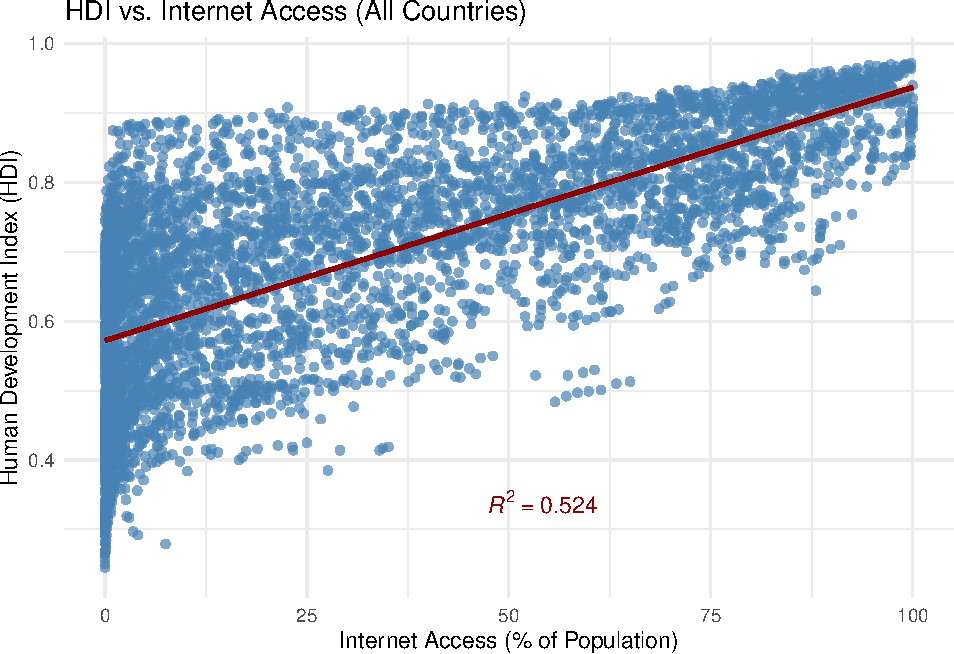
\includegraphics[keepaspectratio]{Exploratory-Data-Analysis_files/figure-latex/ScatterPlots-1.pdf}}

\begin{Shaded}
\begin{Highlighting}[]
\NormalTok{FirstCutDataFiltered }\OtherTok{\textless{}{-}}\NormalTok{ FirstCutData[}\SpecialCharTok{!}\FunctionTok{is.na}\NormalTok{(FirstCutData}\SpecialCharTok{$}\StringTok{\textasciigrave{}}\AttributeTok{Income Group}\StringTok{\textasciigrave{}}\NormalTok{), ]}
\NormalTok{FirstCutDataFiltered}\SpecialCharTok{$}\StringTok{\textasciigrave{}}\AttributeTok{Income Group}\StringTok{\textasciigrave{}} \OtherTok{\textless{}{-}} \FunctionTok{factor}\NormalTok{(}
\NormalTok{  FirstCutDataFiltered}\SpecialCharTok{$}\StringTok{\textasciigrave{}}\AttributeTok{Income Group}\StringTok{\textasciigrave{}}\NormalTok{,}
  \AttributeTok{levels =} \FunctionTok{c}\NormalTok{(}\StringTok{"Low income"}\NormalTok{, }\StringTok{"Lower middle income"}\NormalTok{, }\StringTok{"Upper middle income"}\NormalTok{, }\StringTok{"High income"}\NormalTok{)}
\NormalTok{)}
\FunctionTok{ggplot}\NormalTok{(FirstCutDataFiltered, }\FunctionTok{aes}\NormalTok{(}\AttributeTok{x =}\NormalTok{ InternetUsersPct, }\AttributeTok{y =}\NormalTok{ HDI\_Index, }\AttributeTok{color =} \StringTok{\textasciigrave{}}\AttributeTok{Income Group}\StringTok{\textasciigrave{}}\NormalTok{)) }\SpecialCharTok{+}
  \FunctionTok{geom\_point}\NormalTok{(}\AttributeTok{alpha =} \FloatTok{0.7}\NormalTok{) }\SpecialCharTok{+}
  \FunctionTok{geom\_smooth}\NormalTok{(}\AttributeTok{method =} \StringTok{"lm"}\NormalTok{, }\AttributeTok{se =} \ConstantTok{TRUE}\NormalTok{) }\SpecialCharTok{+}
  \FunctionTok{stat\_poly\_eq}\NormalTok{(}
    \FunctionTok{aes}\NormalTok{(}
      \AttributeTok{label =} \FunctionTok{after\_stat}\NormalTok{(rr.label),}
      \AttributeTok{group =} \StringTok{\textasciigrave{}}\AttributeTok{Income Group}\StringTok{\textasciigrave{}}\NormalTok{,}
      \AttributeTok{color =} \StringTok{\textasciigrave{}}\AttributeTok{Income Group}\StringTok{\textasciigrave{}}
\NormalTok{    ),}
    \AttributeTok{formula =}\NormalTok{ y }\SpecialCharTok{\textasciitilde{}}\NormalTok{ x,}
    \AttributeTok{parse =} \ConstantTok{FALSE}\NormalTok{,}
    \AttributeTok{output.type =} \StringTok{"text"}\NormalTok{,}
    \AttributeTok{rr.digits =} \DecValTok{3}\NormalTok{,}
    \AttributeTok{label.x =} \FloatTok{0.6}\NormalTok{,}
    \AttributeTok{label.y =} \FunctionTok{c}\NormalTok{(}\FloatTok{0.15}\NormalTok{, }\FloatTok{0.2}\NormalTok{, }\FloatTok{0.25}\NormalTok{, }\FloatTok{0.3}\NormalTok{),  }\CommentTok{\# Stack in bottom right}
    \AttributeTok{na.rm =} \ConstantTok{TRUE}
\NormalTok{  ) }\SpecialCharTok{+}
  \FunctionTok{labs}\NormalTok{(}
    \AttributeTok{title =} \StringTok{"HDI vs. Internet Access by Income Group"}\NormalTok{,}
    \AttributeTok{x =} \StringTok{"Internet Access (\% of Population)"}\NormalTok{,}
    \AttributeTok{y =} \StringTok{"Human Development Index (HDI)"}\NormalTok{,}
    \AttributeTok{color =} \StringTok{"Income Group"}
\NormalTok{  ) }\SpecialCharTok{+}
  \FunctionTok{theme\_minimal}\NormalTok{()}
\end{Highlighting}
\end{Shaded}

\begin{verbatim}
## `geom_smooth()` using formula = 'y ~ x'
\end{verbatim}

\begin{verbatim}
## Warning: Removed 646 rows containing non-finite outside the scale range
## (`stat_smooth()`).
\end{verbatim}

\begin{verbatim}
## Warning: Removed 646 rows containing missing values or values outside the scale range
## (`geom_point()`).
\end{verbatim}

\pandocbounded{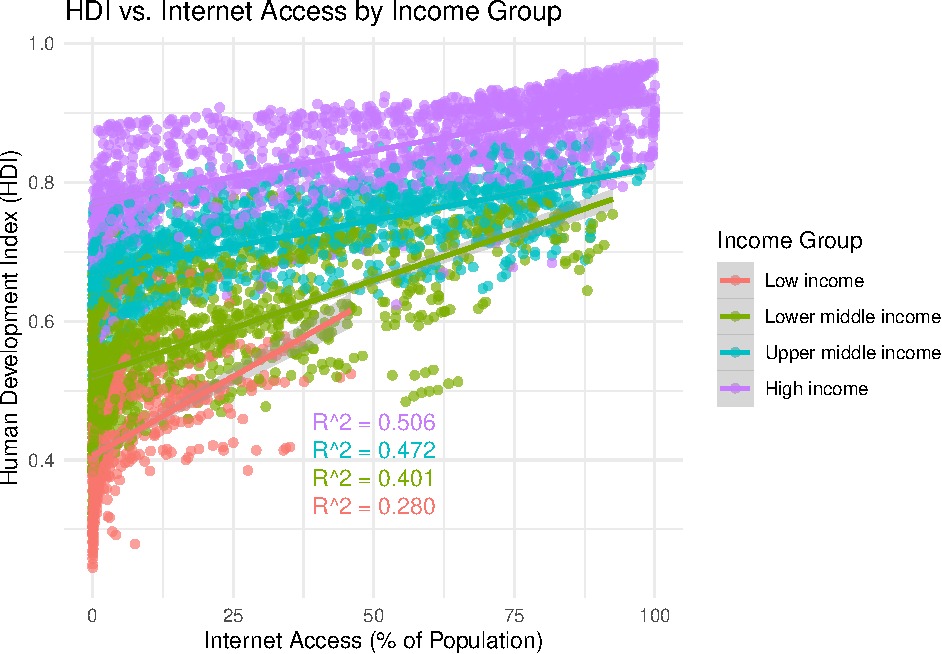
\includegraphics[keepaspectratio]{Exploratory-Data-Analysis_files/figure-latex/ScatterPlots-2.pdf}}

\begin{Shaded}
\begin{Highlighting}[]
\NormalTok{FirstCutDataFiltered }\OtherTok{\textless{}{-}}\NormalTok{ FirstCutData[}\SpecialCharTok{!}\FunctionTok{is.na}\NormalTok{(FirstCutData}\SpecialCharTok{$}\StringTok{\textasciigrave{}}\AttributeTok{Income Group}\StringTok{\textasciigrave{}}\NormalTok{), ]}

\NormalTok{FirstCutDataFiltered}\SpecialCharTok{$}\StringTok{\textasciigrave{}}\AttributeTok{Income Group}\StringTok{\textasciigrave{}} \OtherTok{\textless{}{-}} \FunctionTok{factor}\NormalTok{(}
\NormalTok{  FirstCutDataFiltered}\SpecialCharTok{$}\StringTok{\textasciigrave{}}\AttributeTok{Income Group}\StringTok{\textasciigrave{}}\NormalTok{,}
  \AttributeTok{levels =} \FunctionTok{c}\NormalTok{(}\StringTok{"Low income"}\NormalTok{, }\StringTok{"Lower middle income"}\NormalTok{, }\StringTok{"Upper middle income"}\NormalTok{, }\StringTok{"High income"}\NormalTok{)}
\NormalTok{)}

\NormalTok{FirstCutDataFilteredClean }\OtherTok{\textless{}{-}}\NormalTok{ FirstCutDataFiltered }\SpecialCharTok{\%\textgreater{}\%}
  \FunctionTok{filter}\NormalTok{(}\SpecialCharTok{!}\FunctionTok{is.na}\NormalTok{(InternetUsersPct))}


\FunctionTok{ggplot}\NormalTok{(FirstCutDataFilteredClean, }\FunctionTok{aes}\NormalTok{(}\AttributeTok{x =}\NormalTok{ InternetUsersPct, }\AttributeTok{fill =} \StringTok{\textasciigrave{}}\AttributeTok{Income Group}\StringTok{\textasciigrave{}}\NormalTok{)) }\SpecialCharTok{+}
  \FunctionTok{geom\_histogram}\NormalTok{(}
    \FunctionTok{aes}\NormalTok{(}\AttributeTok{y =} \FunctionTok{after\_stat}\NormalTok{(count }\SpecialCharTok{/} \FunctionTok{tapply}\NormalTok{(count, PANEL, sum)[}\FunctionTok{as.integer}\NormalTok{(PANEL)])),}
    \AttributeTok{binwidth =} \DecValTok{5}\NormalTok{,}
    \AttributeTok{color =} \StringTok{"black"}\NormalTok{,}
    \AttributeTok{alpha =} \FloatTok{0.8}
\NormalTok{  ) }\SpecialCharTok{+}
  \FunctionTok{facet\_wrap}\NormalTok{(}\SpecialCharTok{\textasciitilde{}} \StringTok{\textasciigrave{}}\AttributeTok{Income Group}\StringTok{\textasciigrave{}}\NormalTok{, }\AttributeTok{scales =} \StringTok{"free\_y"}\NormalTok{) }\SpecialCharTok{+}
  \FunctionTok{scale\_y\_continuous}\NormalTok{(}\AttributeTok{labels =}\NormalTok{ scales}\SpecialCharTok{::}\FunctionTok{percent\_format}\NormalTok{(}\AttributeTok{accuracy =} \DecValTok{1}\NormalTok{)) }\SpecialCharTok{+}
  \FunctionTok{scale\_x\_continuous}\NormalTok{(}
    \AttributeTok{breaks =} \FunctionTok{seq}\NormalTok{(}\DecValTok{0}\NormalTok{, }\DecValTok{100}\NormalTok{, }\AttributeTok{by =} \DecValTok{10}\NormalTok{),}
    \AttributeTok{labels =} \ControlFlowTok{function}\NormalTok{(x) }\FunctionTok{paste0}\NormalTok{(x, }\StringTok{"\%"}\NormalTok{)}
\NormalTok{  ) }\SpecialCharTok{+}
  \FunctionTok{labs}\NormalTok{(}
    \AttributeTok{title =} \StringTok{"Distribution of Internet Access by Income Group"}\NormalTok{,}
    \AttributeTok{x =} \StringTok{"Internet Access (\% of Population)"}\NormalTok{,}
    \AttributeTok{y =} \StringTok{"Percent of Observations"}
\NormalTok{  ) }\SpecialCharTok{+}
  \FunctionTok{theme\_minimal}\NormalTok{() }\SpecialCharTok{+}
  \FunctionTok{theme}\NormalTok{(}
    \AttributeTok{strip.text =} \FunctionTok{element\_text}\NormalTok{(}\AttributeTok{face =} \StringTok{"bold"}\NormalTok{),}
    \AttributeTok{axis.text.x =} \FunctionTok{element\_text}\NormalTok{(}\AttributeTok{angle =} \DecValTok{45}\NormalTok{, }\AttributeTok{hjust =} \DecValTok{1}\NormalTok{),}
    \AttributeTok{legend.position =} \StringTok{"none"}
\NormalTok{  )}
\end{Highlighting}
\end{Shaded}

\pandocbounded{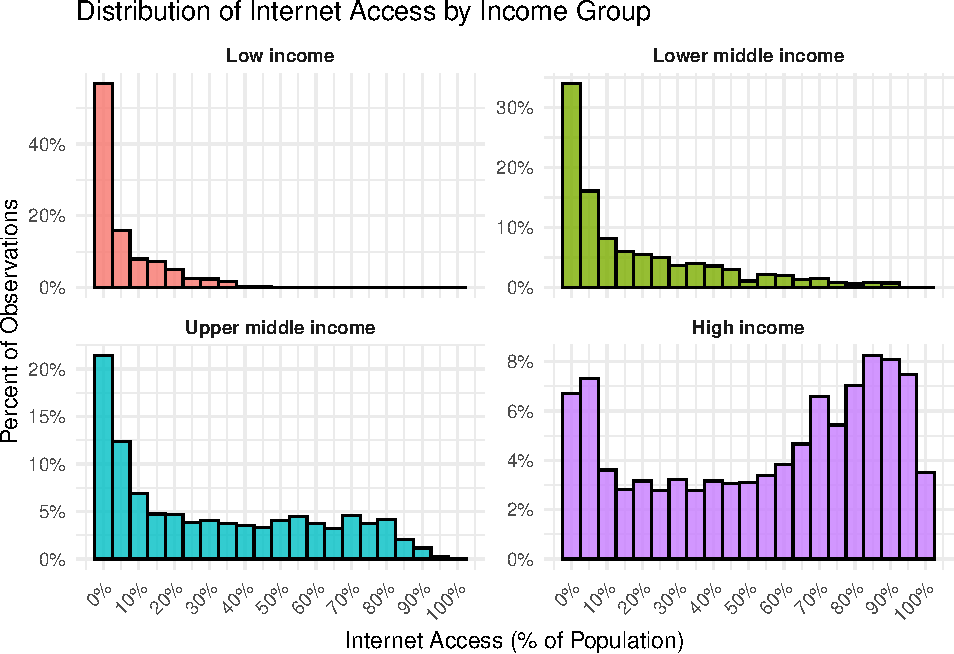
\includegraphics[keepaspectratio]{Exploratory-Data-Analysis_files/figure-latex/InternetDistributionPlots-1.pdf}}

\begin{Shaded}
\begin{Highlighting}[]
\CommentTok{\# Step 1: Filter to only rows with Internet Access under 5\%}
\CommentTok{\# Bin and summarize within the 0\%–5\% range}
\CommentTok{\# Bin and summarize within the 0\%–5\% range}
\NormalTok{zoom\_data }\OtherTok{\textless{}{-}}\NormalTok{ FirstCutDataFiltered }\SpecialCharTok{\%\textgreater{}\%}
  \FunctionTok{filter}\NormalTok{(InternetUsersPct }\SpecialCharTok{\textgreater{}=} \DecValTok{0}\NormalTok{, InternetUsersPct }\SpecialCharTok{\textless{}} \DecValTok{5}\NormalTok{) }\SpecialCharTok{\%\textgreater{}\%}
  \FunctionTok{mutate}\NormalTok{(}\AttributeTok{Bin =} \FunctionTok{cut}\NormalTok{(}
\NormalTok{    InternetUsersPct,}
    \AttributeTok{breaks =} \FunctionTok{seq}\NormalTok{(}\DecValTok{0}\NormalTok{, }\DecValTok{5}\NormalTok{, }\AttributeTok{by =} \DecValTok{1}\NormalTok{),}
    \AttributeTok{include.lowest =} \ConstantTok{TRUE}\NormalTok{,}
    \AttributeTok{right =} \ConstantTok{FALSE}\NormalTok{,}
    \AttributeTok{labels =} \FunctionTok{c}\NormalTok{(}\StringTok{"0–1\%"}\NormalTok{, }\StringTok{"1–2\%"}\NormalTok{, }\StringTok{"2–3\%"}\NormalTok{, }\StringTok{"3–4\%"}\NormalTok{, }\StringTok{"4–5\%"}\NormalTok{)}
\NormalTok{  ))}

\CommentTok{\# Group totals for each Income Group (full data)}
\NormalTok{group\_totals }\OtherTok{\textless{}{-}}\NormalTok{ FirstCutDataFiltered }\SpecialCharTok{\%\textgreater{}\%}
  \FunctionTok{count}\NormalTok{(}\StringTok{\textasciigrave{}}\AttributeTok{Income Group}\StringTok{\textasciigrave{}}\NormalTok{, }\AttributeTok{name =} \StringTok{"GroupTotal"}\NormalTok{)}

\CommentTok{\# Bin counts and percentages}
\NormalTok{zoom\_summary }\OtherTok{\textless{}{-}}\NormalTok{ zoom\_data }\SpecialCharTok{\%\textgreater{}\%}
  \FunctionTok{count}\NormalTok{(}\StringTok{\textasciigrave{}}\AttributeTok{Income Group}\StringTok{\textasciigrave{}}\NormalTok{, Bin, }\AttributeTok{name =} \StringTok{"BinCount"}\NormalTok{) }\SpecialCharTok{\%\textgreater{}\%}
  \FunctionTok{left\_join}\NormalTok{(group\_totals, }\AttributeTok{by =} \StringTok{"Income Group"}\NormalTok{) }\SpecialCharTok{\%\textgreater{}\%}
  \FunctionTok{mutate}\NormalTok{(}\AttributeTok{Percent =}\NormalTok{ BinCount }\SpecialCharTok{/}\NormalTok{ GroupTotal)}

\CommentTok{\# Plot}
\FunctionTok{ggplot}\NormalTok{(zoom\_summary, }\FunctionTok{aes}\NormalTok{(}\AttributeTok{x =}\NormalTok{ Bin, }\AttributeTok{y =}\NormalTok{ Percent, }\AttributeTok{fill =} \StringTok{\textasciigrave{}}\AttributeTok{Income Group}\StringTok{\textasciigrave{}}\NormalTok{)) }\SpecialCharTok{+}
  \FunctionTok{geom\_col}\NormalTok{(}\AttributeTok{color =} \StringTok{"black"}\NormalTok{, }\AttributeTok{width =} \FloatTok{0.9}\NormalTok{) }\SpecialCharTok{+}
  \FunctionTok{facet\_wrap}\NormalTok{(}\SpecialCharTok{\textasciitilde{}} \StringTok{\textasciigrave{}}\AttributeTok{Income Group}\StringTok{\textasciigrave{}}\NormalTok{, }\AttributeTok{scales =} \StringTok{"free\_y"}\NormalTok{) }\SpecialCharTok{+}
  \FunctionTok{scale\_y\_continuous}\NormalTok{(}\AttributeTok{labels =}\NormalTok{ scales}\SpecialCharTok{::}\FunctionTok{percent\_format}\NormalTok{(}\AttributeTok{accuracy =} \DecValTok{1}\NormalTok{)) }\SpecialCharTok{+}
  \FunctionTok{labs}\NormalTok{(}
    \AttributeTok{title =} \StringTok{"Zoomed View: Internet Access Below 5\% by Income Group"}\NormalTok{,}
    \AttributeTok{x =} \StringTok{"Internet Access (\% of Population)"}\NormalTok{,}
    \AttributeTok{y =} \StringTok{"Percent of Observations"}
\NormalTok{  ) }\SpecialCharTok{+}
  \FunctionTok{theme\_minimal}\NormalTok{() }\SpecialCharTok{+}
  \FunctionTok{theme}\NormalTok{(}
    \AttributeTok{strip.text =} \FunctionTok{element\_text}\NormalTok{(}\AttributeTok{face =} \StringTok{"bold"}\NormalTok{, }\AttributeTok{size =} \DecValTok{12}\NormalTok{),}
    \AttributeTok{axis.text.x =} \FunctionTok{element\_text}\NormalTok{(}\AttributeTok{angle =} \DecValTok{0}\NormalTok{, }\AttributeTok{hjust =} \FloatTok{0.5}\NormalTok{),}
    \AttributeTok{legend.position =} \StringTok{"none"}
\NormalTok{  ) }
\end{Highlighting}
\end{Shaded}

\pandocbounded{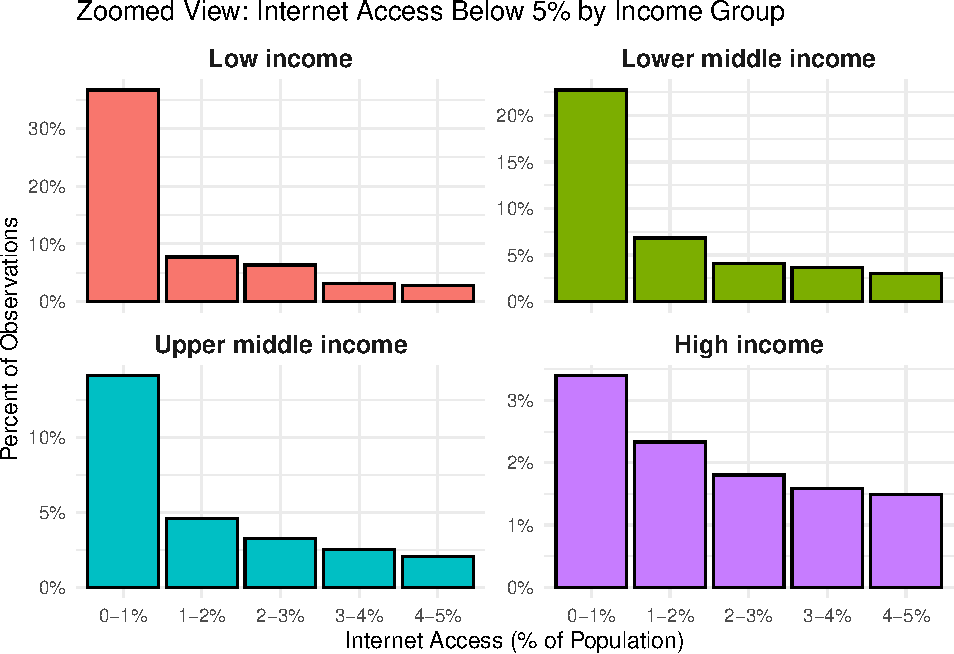
\includegraphics[keepaspectratio]{Exploratory-Data-Analysis_files/figure-latex/InternetDistributionPlots-2.pdf}}

\begin{Shaded}
\begin{Highlighting}[]
\FunctionTok{ggplot}\NormalTok{(FirstCutDataFiltered, }\FunctionTok{aes}\NormalTok{(}\AttributeTok{x =} \StringTok{\textasciigrave{}}\AttributeTok{Income Group}\StringTok{\textasciigrave{}}\NormalTok{, }\AttributeTok{y =}\NormalTok{ HDI\_Index, }\AttributeTok{fill =} \StringTok{\textasciigrave{}}\AttributeTok{Income Group}\StringTok{\textasciigrave{}}\NormalTok{)) }\SpecialCharTok{+}
  \FunctionTok{geom\_violin}\NormalTok{(}\AttributeTok{trim =} \ConstantTok{FALSE}\NormalTok{, }\AttributeTok{alpha =} \FloatTok{0.7}\NormalTok{) }\SpecialCharTok{+}
  \FunctionTok{geom\_jitter}\NormalTok{(}\AttributeTok{width =} \FloatTok{0.15}\NormalTok{, }\AttributeTok{alpha =} \FloatTok{0.3}\NormalTok{, }\AttributeTok{color =} \StringTok{"black"}\NormalTok{, }\AttributeTok{size =} \DecValTok{1}\NormalTok{) }\SpecialCharTok{+}
  \FunctionTok{labs}\NormalTok{(}
    \AttributeTok{title =} \StringTok{"Distribution of HDI by Income Group"}\NormalTok{,}
    \AttributeTok{x =} \StringTok{"Income Group"}\NormalTok{,}
    \AttributeTok{y =} \StringTok{"Human Development Index (HDI)"}
\NormalTok{  ) }\SpecialCharTok{+}
  \FunctionTok{theme\_minimal}\NormalTok{(}\AttributeTok{base\_size =} \DecValTok{14}\NormalTok{) }\SpecialCharTok{+}
  \FunctionTok{theme}\NormalTok{(}
    \AttributeTok{legend.position =} \StringTok{"none"}\NormalTok{,}
    \AttributeTok{plot.title =} \FunctionTok{element\_text}\NormalTok{(}\AttributeTok{face =} \StringTok{"bold"}\NormalTok{),}
    \AttributeTok{axis.title.x =} \FunctionTok{element\_text}\NormalTok{(}\AttributeTok{face =} \StringTok{"bold"}\NormalTok{),}
    \AttributeTok{axis.title.y =} \FunctionTok{element\_text}\NormalTok{(}\AttributeTok{face =} \StringTok{"bold"}\NormalTok{)}
\NormalTok{  )}
\end{Highlighting}
\end{Shaded}

\begin{verbatim}
## Warning: Removed 417 rows containing non-finite outside the scale range
## (`stat_ydensity()`).
\end{verbatim}

\begin{verbatim}
## Warning: Removed 417 rows containing missing values or values outside the scale range
## (`geom_point()`).
\end{verbatim}

\pandocbounded{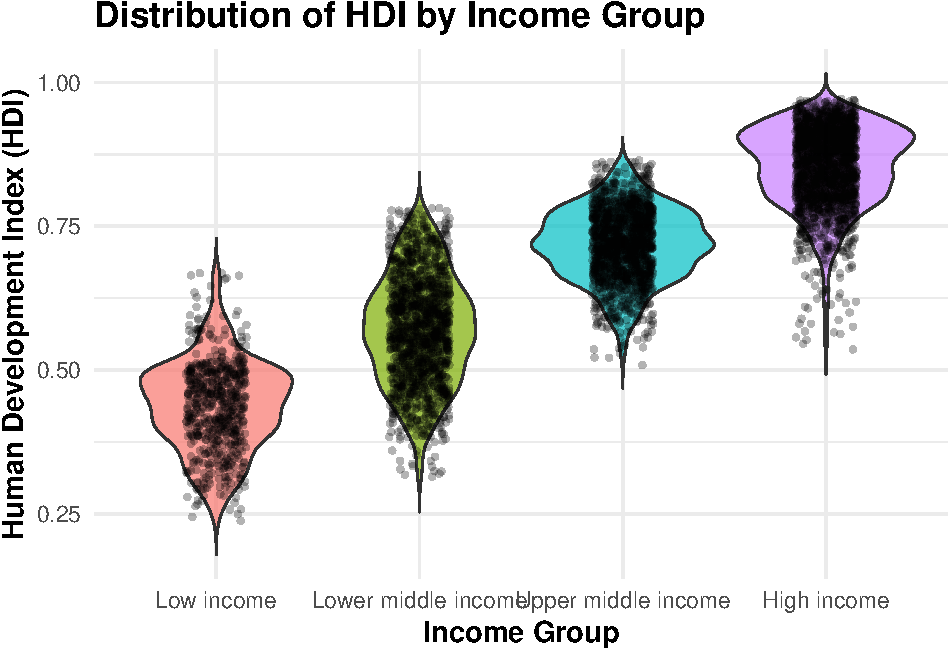
\includegraphics[keepaspectratio]{Exploratory-Data-Analysis_files/figure-latex/ViolinPlots-1.pdf}}

\begin{Shaded}
\begin{Highlighting}[]
\FunctionTok{ggplot}\NormalTok{(FirstCutDataFiltered, }\FunctionTok{aes}\NormalTok{(}\AttributeTok{x =} \StringTok{\textasciigrave{}}\AttributeTok{Income Group}\StringTok{\textasciigrave{}}\NormalTok{, }\AttributeTok{y =}\NormalTok{ InternetUsersPct, }\AttributeTok{fill =} \StringTok{\textasciigrave{}}\AttributeTok{Income Group}\StringTok{\textasciigrave{}}\NormalTok{)) }\SpecialCharTok{+}
  \FunctionTok{geom\_violin}\NormalTok{(}\AttributeTok{trim =} \ConstantTok{TRUE}\NormalTok{, }\AttributeTok{color =} \StringTok{"black"}\NormalTok{, }\AttributeTok{adjust =} \FloatTok{1.2}\NormalTok{) }\SpecialCharTok{+}  \CommentTok{\# trim removes tails beyond the data}
  \FunctionTok{geom\_jitter}\NormalTok{(}\AttributeTok{width =} \FloatTok{0.2}\NormalTok{, }\AttributeTok{size =} \DecValTok{1}\NormalTok{, }\AttributeTok{alpha =} \FloatTok{0.5}\NormalTok{, }\AttributeTok{color =} \StringTok{"black"}\NormalTok{) }\SpecialCharTok{+}
  \FunctionTok{scale\_y\_continuous}\NormalTok{(}\AttributeTok{limits =} \FunctionTok{c}\NormalTok{(}\DecValTok{0}\NormalTok{, }\DecValTok{100}\NormalTok{), }\AttributeTok{expand =} \FunctionTok{c}\NormalTok{(}\DecValTok{0}\NormalTok{, }\DecValTok{0}\NormalTok{)) }\SpecialCharTok{+}  \CommentTok{\# Hard clip y{-}axis}
  \FunctionTok{labs}\NormalTok{(}
    \AttributeTok{title =} \StringTok{"Distribution of Internet Access by Income Group"}\NormalTok{,}
    \AttributeTok{y =} \StringTok{"Internet Access (\% of Population)"}\NormalTok{,}
    \AttributeTok{x =} \StringTok{"Income Group"}
\NormalTok{  ) }\SpecialCharTok{+}
  \FunctionTok{theme\_minimal}\NormalTok{() }\SpecialCharTok{+}
  \FunctionTok{theme}\NormalTok{(}
    \AttributeTok{plot.title =} \FunctionTok{element\_text}\NormalTok{(}\AttributeTok{hjust =} \FloatTok{0.5}\NormalTok{, }\AttributeTok{face =} \StringTok{"bold"}\NormalTok{),}
    \AttributeTok{axis.title =} \FunctionTok{element\_text}\NormalTok{(}\AttributeTok{face =} \StringTok{"bold"}\NormalTok{),}
    \AttributeTok{axis.text.x =} \FunctionTok{element\_text}\NormalTok{(}\AttributeTok{face =} \StringTok{"bold"}\NormalTok{),}
    \AttributeTok{legend.position =} \StringTok{"none"}
\NormalTok{  ) }\SpecialCharTok{+}
  \FunctionTok{scale\_fill\_manual}\NormalTok{(}\AttributeTok{values =} \FunctionTok{c}\NormalTok{(}
    \StringTok{"Low income"} \OtherTok{=} \StringTok{"\#F8766D"}\NormalTok{,}
    \StringTok{"Lower middle income"} \OtherTok{=} \StringTok{"\#7CAE00"}\NormalTok{,}
    \StringTok{"Upper middle income"} \OtherTok{=} \StringTok{"\#00BFC4"}\NormalTok{,}
    \StringTok{"High income"} \OtherTok{=} \StringTok{"\#C77CFF"}
\NormalTok{  ))}
\end{Highlighting}
\end{Shaded}

\begin{verbatim}
## Warning: Removed 348 rows containing non-finite outside the scale range
## (`stat_ydensity()`).
\end{verbatim}

\begin{verbatim}
## Warning: Removed 370 rows containing missing values or values outside the scale range
## (`geom_point()`).
\end{verbatim}

\pandocbounded{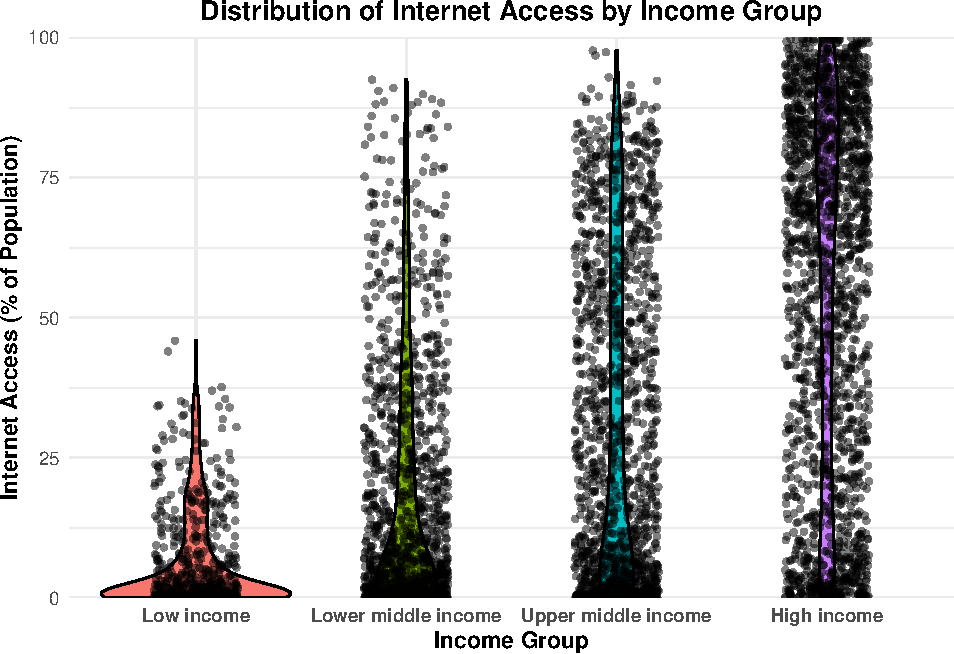
\includegraphics[keepaspectratio]{Exploratory-Data-Analysis_files/figure-latex/ViolinPlots-2.pdf}}

\begin{Shaded}
\begin{Highlighting}[]
\CommentTok{\# Step 1: Select only numeric columns and drop unwanted ones}
\NormalTok{numeric\_vars }\OtherTok{\textless{}{-}}\NormalTok{ FirstCutData }\SpecialCharTok{\%\textgreater{}\%}
  \FunctionTok{select}\NormalTok{(}\FunctionTok{where}\NormalTok{(is.numeric)) }\SpecialCharTok{\%\textgreater{}\%}
  \FunctionTok{select}\NormalTok{(}\SpecialCharTok{{-}}\NormalTok{year)  }\CommentTok{\# Drop the \textquotesingle{}Year\textquotesingle{} column}

\CommentTok{\# Step 2: Compute correlation matrix using pairwise complete observations}
\NormalTok{cor\_matrix }\OtherTok{\textless{}{-}} \FunctionTok{cor}\NormalTok{(numeric\_vars, }\AttributeTok{use =} \StringTok{"pairwise.complete.obs"}\NormalTok{, }\AttributeTok{method =} \StringTok{"pearson"}\NormalTok{)}
\NormalTok{cor\_matrix\_90 }\OtherTok{\textless{}{-}} \FunctionTok{ifelse}\NormalTok{(}\FunctionTok{abs}\NormalTok{(cor\_matrix) }\SpecialCharTok{\textgreater{}=} \FloatTok{0.9}\NormalTok{, cor\_matrix, }\ConstantTok{NA}\NormalTok{)}
\NormalTok{cor\_matrix\_70\_90 }\OtherTok{\textless{}{-}} \FunctionTok{ifelse}\NormalTok{(}\FunctionTok{abs}\NormalTok{(cor\_matrix) }\SpecialCharTok{\textgreater{}=} \FloatTok{0.7} \SpecialCharTok{\&} \FunctionTok{abs}\NormalTok{(cor\_matrix) }\SpecialCharTok{\textless{}} \FloatTok{0.9}\NormalTok{, cor\_matrix, }\ConstantTok{NA}\NormalTok{)}


\CommentTok{\# Step 3: Plot correlation heatmap}
\FunctionTok{corrplot}\NormalTok{(cor\_matrix,}
         \AttributeTok{method =} \StringTok{"color"}\NormalTok{,}
         \AttributeTok{type =} \StringTok{"lower"}\NormalTok{,}
         \AttributeTok{tl.col =} \StringTok{"black"}\NormalTok{,}
         \AttributeTok{tl.cex =} \FloatTok{0.7}\NormalTok{,}
         \AttributeTok{col =} \FunctionTok{colorRampPalette}\NormalTok{(}\FunctionTok{c}\NormalTok{(}\StringTok{"blue"}\NormalTok{, }\StringTok{"white"}\NormalTok{, }\StringTok{"red"}\NormalTok{))(}\DecValTok{200}\NormalTok{),}
         \AttributeTok{diag =} \ConstantTok{FALSE}\NormalTok{)}
\FunctionTok{title}\NormalTok{(}\StringTok{"Correlation Heatmap of Numeric Predictors {-} ALL"}\NormalTok{, }\AttributeTok{line =} \DecValTok{1}\NormalTok{, }\AttributeTok{cex.main =} \FloatTok{1.2}\NormalTok{)}
\end{Highlighting}
\end{Shaded}

\pandocbounded{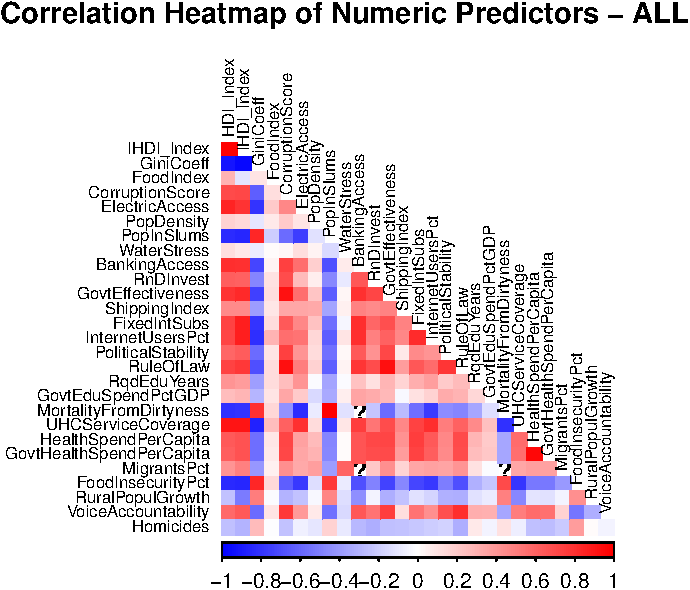
\includegraphics[keepaspectratio]{Exploratory-Data-Analysis_files/figure-latex/Correlation-1.pdf}}

\begin{Shaded}
\begin{Highlighting}[]
\CommentTok{\# Plot only strong correlations}
\FunctionTok{corrplot}\NormalTok{(cor\_matrix\_90,}
         \AttributeTok{method =} \StringTok{"color"}\NormalTok{,}
         \AttributeTok{type =} \StringTok{"lower"}\NormalTok{,}
         \AttributeTok{tl.col =} \StringTok{"black"}\NormalTok{,}
         \AttributeTok{tl.cex =} \FloatTok{0.7}\NormalTok{,}
         \AttributeTok{col =} \FunctionTok{colorRampPalette}\NormalTok{(}\FunctionTok{c}\NormalTok{(}\StringTok{"blue"}\NormalTok{, }\StringTok{"white"}\NormalTok{, }\StringTok{"red"}\NormalTok{))(}\DecValTok{200}\NormalTok{),}
         \AttributeTok{diag =} \ConstantTok{FALSE}\NormalTok{,}
         \AttributeTok{na.label =} \StringTok{" "}\NormalTok{)  }\CommentTok{\# blank for missing (non{-}displayed) values}
\FunctionTok{title}\NormalTok{(}\StringTok{"Correlation Heatmap of Numeric Predictors {-} 90\%+ correlation (DROP)"}\NormalTok{, }\AttributeTok{line =} \DecValTok{1}\NormalTok{, }\AttributeTok{cex.main =} \FloatTok{1.2}\NormalTok{)}
\end{Highlighting}
\end{Shaded}

\pandocbounded{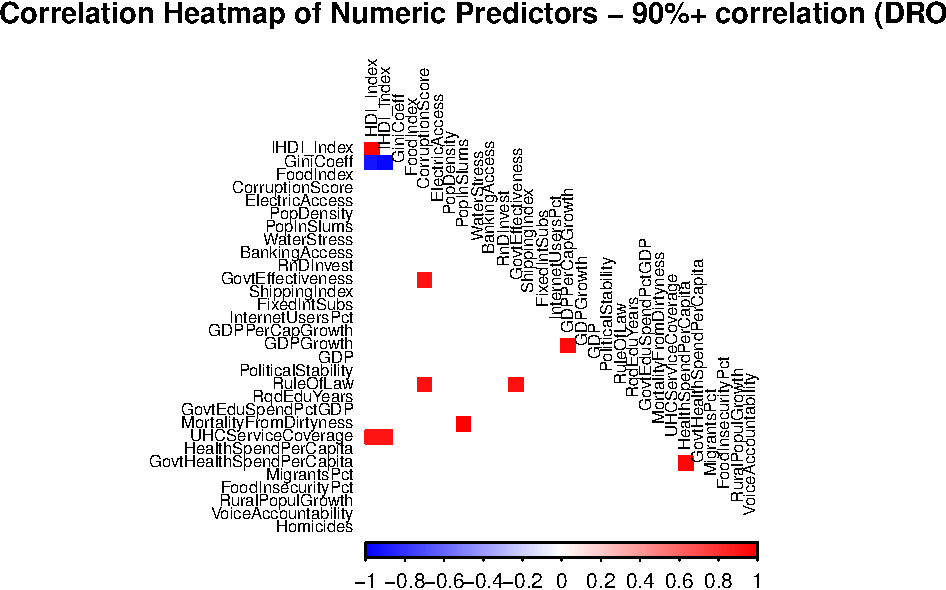
\includegraphics[keepaspectratio]{Exploratory-Data-Analysis_files/figure-latex/Correlation-2.pdf}}

\begin{Shaded}
\begin{Highlighting}[]
\FunctionTok{corrplot}\NormalTok{(cor\_matrix\_70\_90,}
         \AttributeTok{method =} \StringTok{"color"}\NormalTok{,}
         \AttributeTok{type =} \StringTok{"lower"}\NormalTok{,}
         \AttributeTok{tl.col =} \StringTok{"black"}\NormalTok{,}
         \AttributeTok{tl.cex =} \FloatTok{0.7}\NormalTok{,}
         \AttributeTok{col =} \FunctionTok{colorRampPalette}\NormalTok{(}\FunctionTok{c}\NormalTok{(}\StringTok{"blue"}\NormalTok{, }\StringTok{"white"}\NormalTok{, }\StringTok{"red"}\NormalTok{))(}\DecValTok{200}\NormalTok{),}
         \AttributeTok{diag =} \ConstantTok{FALSE}\NormalTok{,}
         \AttributeTok{na.label =} \StringTok{" "}\NormalTok{)  }\CommentTok{\# blank for missing (non{-}displayed) values}
\FunctionTok{title}\NormalTok{(}\StringTok{"Correlation Heatmap of Numeric Predictors {-} 70\%{-}90\%+ correlation (VIF)"}\NormalTok{, }\AttributeTok{line =} \DecValTok{1}\NormalTok{, }\AttributeTok{cex.main =} \FloatTok{1.2}\NormalTok{)}
\end{Highlighting}
\end{Shaded}

\pandocbounded{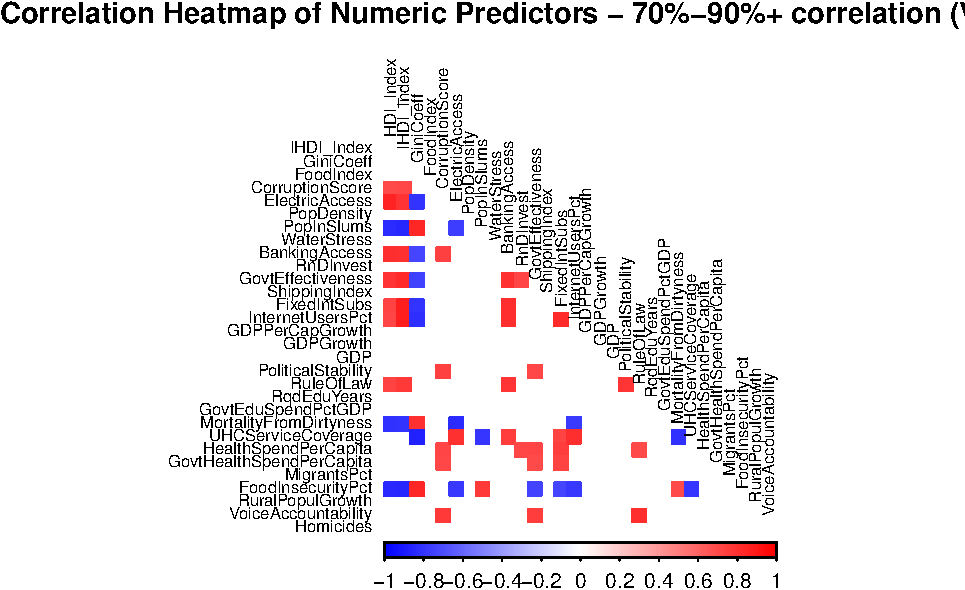
\includegraphics[keepaspectratio]{Exploratory-Data-Analysis_files/figure-latex/Correlation-3.pdf}}

\begin{Shaded}
\begin{Highlighting}[]
\CommentTok{\# Step 2: Compute Pearson correlation matrix using pairwise complete observations}
\NormalTok{cor\_matrix }\OtherTok{\textless{}{-}} \FunctionTok{cor}\NormalTok{(numeric\_vars, }\AttributeTok{use =} \StringTok{"pairwise.complete.obs"}\NormalTok{, }\AttributeTok{method =} \StringTok{"pearson"}\NormalTok{)}

\CommentTok{\# Step 3 Print}
\CommentTok{\# Get total number of columns}
\NormalTok{cols }\OtherTok{\textless{}{-}} \FunctionTok{ncol}\NormalTok{(cor\_matrix)}
\NormalTok{col\_names }\OtherTok{\textless{}{-}} \FunctionTok{colnames}\NormalTok{(cor\_matrix)}

\CommentTok{\# Loop through and print in chunks}
\ControlFlowTok{for}\NormalTok{ (i }\ControlFlowTok{in} \FunctionTok{seq}\NormalTok{(}\DecValTok{1}\NormalTok{, cols, }\AttributeTok{by =}\NormalTok{ cols\_per\_table)) \{}
  \CommentTok{\# Subset the matrix}
\NormalTok{  end\_col }\OtherTok{\textless{}{-}} \FunctionTok{min}\NormalTok{(i }\SpecialCharTok{+}\NormalTok{ cols\_per\_table }\SpecialCharTok{{-}} \DecValTok{1}\NormalTok{, cols)}
\NormalTok{  sub\_matrix }\OtherTok{\textless{}{-}}\NormalTok{ cor\_matrix[, i}\SpecialCharTok{:}\NormalTok{end\_col]}
  
  \CommentTok{\# Print each chunk with a dynamic caption}
  \FunctionTok{cat}\NormalTok{(}
    \FunctionTok{asis\_output}\NormalTok{(}
      \FunctionTok{kable}\NormalTok{(}
        \FunctionTok{round}\NormalTok{(sub\_matrix, }\DecValTok{2}\NormalTok{), }
        \AttributeTok{format =} \StringTok{"latex"}\NormalTok{, }
        \AttributeTok{booktabs =} \ConstantTok{TRUE}\NormalTok{,}
        \AttributeTok{caption =} \FunctionTok{paste0}\NormalTok{(}\StringTok{"Correlation Matrix: Columns "}\NormalTok{, i, }\StringTok{" to "}\NormalTok{, end\_col)) }\SpecialCharTok{\%\textgreater{}\%}
        \FunctionTok{kable\_styling}\NormalTok{(}\AttributeTok{latex\_options =} \FunctionTok{c}\NormalTok{(}\StringTok{"HOLD\_Position"}\NormalTok{, }\StringTok{"striped"}\NormalTok{, }\StringTok{"scale\_down"}\NormalTok{))}
\NormalTok{      )}
\NormalTok{  )}
\NormalTok{\}}
\end{Highlighting}
\end{Shaded}

\begin{table}
\centering
\caption{\label{tab:Correlation}Correlation Matrix: Columns 1 to 8}
\centering
\resizebox{\ifdim\width>\linewidth\linewidth\else\width\fi}{!}{
\begin{tabular}[t]{lrrrrrrrr}
\toprule
  & HDI\_Index & IHDI\_Index & GiniCoeff & FoodIndex & CorruptionScore & ElectricAccess & PopDensity & PopInSlums\\
\midrule
\cellcolor{gray!10}{HDI\_Index} & \cellcolor{gray!10}{1.00} & \cellcolor{gray!10}{0.98} & \cellcolor{gray!10}{-0.92} & \cellcolor{gray!10}{0.29} & \cellcolor{gray!10}{0.71} & \cellcolor{gray!10}{0.85} & \cellcolor{gray!10}{0.17} & \cellcolor{gray!10}{-0.82}\\
IHDI\_Index & 0.98 & 1.00 & -0.97 & -0.10 & 0.72 & 0.80 & 0.14 & -0.85\\
\cellcolor{gray!10}{GiniCoeff} & \cellcolor{gray!10}{-0.92} & \cellcolor{gray!10}{-0.97} & \cellcolor{gray!10}{1.00} & \cellcolor{gray!10}{0.10} & \cellcolor{gray!10}{-0.62} & \cellcolor{gray!10}{-0.79} & \cellcolor{gray!10}{-0.09} & \cellcolor{gray!10}{0.84}\\
FoodIndex & 0.29 & -0.10 & 0.10 & 1.00 & 0.13 & 0.20 & 0.08 & -0.20\\
\cellcolor{gray!10}{CorruptionScore} & \cellcolor{gray!10}{0.71} & \cellcolor{gray!10}{0.72} & \cellcolor{gray!10}{-0.62} & \cellcolor{gray!10}{0.13} & \cellcolor{gray!10}{1.00} & \cellcolor{gray!10}{0.47} & \cellcolor{gray!10}{0.20} & \cellcolor{gray!10}{-0.57}\\
\addlinespace
ElectricAccess & 0.85 & 0.80 & -0.79 & 0.20 & 0.47 & 1.00 & 0.10 & -0.75\\
\cellcolor{gray!10}{PopDensity} & \cellcolor{gray!10}{0.17} & \cellcolor{gray!10}{0.14} & \cellcolor{gray!10}{-0.09} & \cellcolor{gray!10}{0.08} & \cellcolor{gray!10}{0.20} & \cellcolor{gray!10}{0.10} & \cellcolor{gray!10}{1.00} & \cellcolor{gray!10}{-0.11}\\
PopInSlums & -0.82 & -0.85 & 0.84 & -0.20 & -0.57 & -0.75 & -0.11 & 1.00\\
\cellcolor{gray!10}{WaterStress} & \cellcolor{gray!10}{0.12} & \cellcolor{gray!10}{0.08} & \cellcolor{gray!10}{-0.08} & \cellcolor{gray!10}{0.01} & \cellcolor{gray!10}{0.04} & \cellcolor{gray!10}{0.13} & \cellcolor{gray!10}{0.05} & \cellcolor{gray!10}{-0.14}\\
BankingAccess & 0.82 & 0.81 & -0.72 & 0.04 & 0.75 & 0.56 & 0.18 & -0.69\\
\addlinespace
\cellcolor{gray!10}{RnDInvest} & \cellcolor{gray!10}{0.63} & \cellcolor{gray!10}{0.62} & \cellcolor{gray!10}{-0.47} & \cellcolor{gray!10}{0.12} & \cellcolor{gray!10}{0.69} & \cellcolor{gray!10}{0.27} & \cellcolor{gray!10}{0.07} & \cellcolor{gray!10}{-0.47}\\
GovtEffectiveness & 0.79 & 0.83 & -0.74 & 0.12 & 0.92 & 0.57 & 0.22 & -0.64\\
\cellcolor{gray!10}{ShippingIndex} & \cellcolor{gray!10}{0.46} & \cellcolor{gray!10}{0.46} & \cellcolor{gray!10}{-0.38} & \cellcolor{gray!10}{0.10} & \cellcolor{gray!10}{0.35} & \cellcolor{gray!10}{0.34} & \cellcolor{gray!10}{0.34} & \cellcolor{gray!10}{-0.36}\\
FixedIntSubs & 0.73 & 0.88 & -0.80 & 0.14 & 0.64 & 0.47 & 0.24 & -0.57\\
\cellcolor{gray!10}{InternetUsersPct} & \cellcolor{gray!10}{0.72} & \cellcolor{gray!10}{0.87} & \cellcolor{gray!10}{-0.82} & \cellcolor{gray!10}{0.29} & \cellcolor{gray!10}{0.56} & \cellcolor{gray!10}{0.55} & \cellcolor{gray!10}{0.15} & \cellcolor{gray!10}{-0.64}\\
\addlinespace
PoliticalStability & 0.59 & 0.63 & -0.58 & 0.10 & 0.75 & 0.41 & 0.14 & -0.56\\
\cellcolor{gray!10}{RuleOfLaw} & \cellcolor{gray!10}{0.74} & \cellcolor{gray!10}{0.77} & \cellcolor{gray!10}{-0.68} & \cellcolor{gray!10}{0.13} & \cellcolor{gray!10}{0.94} & \cellcolor{gray!10}{0.50} & \cellcolor{gray!10}{0.18} & \cellcolor{gray!10}{-0.63}\\
RqdEduYears & 0.41 & 0.39 & -0.38 & 0.13 & 0.26 & 0.42 & -0.01 & -0.36\\
\cellcolor{gray!10}{GovtEduSpendPctGDP} & \cellcolor{gray!10}{0.26} & \cellcolor{gray!10}{0.28} & \cellcolor{gray!10}{-0.28} & \cellcolor{gray!10}{0.11} & \cellcolor{gray!10}{0.35} & \cellcolor{gray!10}{0.20} & \cellcolor{gray!10}{-0.15} & \cellcolor{gray!10}{-0.33}\\
MortalityFromDirtyness & -0.80 & -0.79 & 0.80 & 0.15 & -0.42 & -0.82 & -0.07 & 1.00\\
\addlinespace
\cellcolor{gray!10}{UHCServiceCoverage} & \cellcolor{gray!10}{0.92} & \cellcolor{gray!10}{0.92} & \cellcolor{gray!10}{-0.86} & \cellcolor{gray!10}{0.25} & \cellcolor{gray!10}{0.61} & \cellcolor{gray!10}{0.81} & \cellcolor{gray!10}{0.13} & \cellcolor{gray!10}{-0.79}\\
HealthSpendPerCapita & 0.64 & 0.68 & -0.57 & 0.09 & 0.73 & 0.36 & 0.26 & -0.48\\
\cellcolor{gray!10}{GovtHealthSpendPerCapita} & \cellcolor{gray!10}{0.63} & \cellcolor{gray!10}{0.67} & \cellcolor{gray!10}{-0.57} & \cellcolor{gray!10}{0.09} & \cellcolor{gray!10}{0.72} & \cellcolor{gray!10}{0.35} & \cellcolor{gray!10}{0.29} & \cellcolor{gray!10}{-0.47}\\
MigrantsPct & 0.41 & 0.50 & -0.41 & 0.06 & 0.43 & 0.34 & 0.37 & -0.38\\
\cellcolor{gray!10}{FoodInsecurityPct} & \cellcolor{gray!10}{-0.83} & \cellcolor{gray!10}{-0.85} & \cellcolor{gray!10}{0.84} & \cellcolor{gray!10}{0.14} & \cellcolor{gray!10}{-0.62} & \cellcolor{gray!10}{-0.78} & \cellcolor{gray!10}{-0.13} & \cellcolor{gray!10}{0.77}\\
\addlinespace
RuralPopulGrowth & -0.24 & -0.52 & 0.50 & -0.02 & -0.30 & -0.23 & -0.03 & 0.48\\
\cellcolor{gray!10}{VoiceAccountability} & \cellcolor{gray!10}{0.59} & \cellcolor{gray!10}{0.65} & \cellcolor{gray!10}{-0.58} & \cellcolor{gray!10}{0.10} & \cellcolor{gray!10}{0.77} & \cellcolor{gray!10}{0.40} & \cellcolor{gray!10}{0.08} & \cellcolor{gray!10}{-0.55}\\
Homicides & -0.24 & -0.30 & 0.26 & -0.01 & -0.24 & -0.06 & -0.09 & 0.17\\
\bottomrule
\end{tabular}}
\end{table}\begin{table}
\centering
\caption{\label{tab:Correlation}Correlation Matrix: Columns 9 to 16}
\centering
\resizebox{\ifdim\width>\linewidth\linewidth\else\width\fi}{!}{
\begin{tabular}[t]{lrrrrrrrr}
\toprule
  & WaterStress & BankingAccess & RnDInvest & GovtEffectiveness & ShippingIndex & FixedIntSubs & InternetUsersPct & PoliticalStability\\
\midrule
\cellcolor{gray!10}{HDI\_Index} & \cellcolor{gray!10}{0.12} & \cellcolor{gray!10}{0.82} & \cellcolor{gray!10}{0.63} & \cellcolor{gray!10}{0.79} & \cellcolor{gray!10}{0.46} & \cellcolor{gray!10}{0.73} & \cellcolor{gray!10}{0.72} & \cellcolor{gray!10}{0.59}\\
IHDI\_Index & 0.08 & 0.81 & 0.62 & 0.83 & 0.46 & 0.88 & 0.87 & 0.63\\
\cellcolor{gray!10}{GiniCoeff} & \cellcolor{gray!10}{-0.08} & \cellcolor{gray!10}{-0.72} & \cellcolor{gray!10}{-0.47} & \cellcolor{gray!10}{-0.74} & \cellcolor{gray!10}{-0.38} & \cellcolor{gray!10}{-0.80} & \cellcolor{gray!10}{-0.82} & \cellcolor{gray!10}{-0.58}\\
FoodIndex & 0.01 & 0.04 & 0.12 & 0.12 & 0.10 & 0.14 & 0.29 & 0.10\\
\cellcolor{gray!10}{CorruptionScore} & \cellcolor{gray!10}{0.04} & \cellcolor{gray!10}{0.75} & \cellcolor{gray!10}{0.69} & \cellcolor{gray!10}{0.92} & \cellcolor{gray!10}{0.35} & \cellcolor{gray!10}{0.64} & \cellcolor{gray!10}{0.56} & \cellcolor{gray!10}{0.75}\\
\addlinespace
ElectricAccess & 0.13 & 0.56 & 0.27 & 0.57 & 0.34 & 0.47 & 0.55 & 0.41\\
\cellcolor{gray!10}{PopDensity} & \cellcolor{gray!10}{0.05} & \cellcolor{gray!10}{0.18} & \cellcolor{gray!10}{0.07} & \cellcolor{gray!10}{0.22} & \cellcolor{gray!10}{0.34} & \cellcolor{gray!10}{0.24} & \cellcolor{gray!10}{0.15} & \cellcolor{gray!10}{0.14}\\
PopInSlums & -0.14 & -0.69 & -0.47 & -0.64 & -0.36 & -0.57 & -0.64 & -0.56\\
\cellcolor{gray!10}{WaterStress} & \cellcolor{gray!10}{1.00} & \cellcolor{gray!10}{0.08} & \cellcolor{gray!10}{-0.08} & \cellcolor{gray!10}{0.04} & \cellcolor{gray!10}{0.05} & \cellcolor{gray!10}{-0.04} & \cellcolor{gray!10}{0.10} & \cellcolor{gray!10}{0.03}\\
BankingAccess & 0.08 & 1.00 & 0.66 & 0.80 & 0.49 & 0.81 & 0.81 & 0.65\\
\addlinespace
\cellcolor{gray!10}{RnDInvest} & \cellcolor{gray!10}{-0.08} & \cellcolor{gray!10}{0.66} & \cellcolor{gray!10}{1.00} & \cellcolor{gray!10}{0.72} & \cellcolor{gray!10}{0.46} & \cellcolor{gray!10}{0.59} & \cellcolor{gray!10}{0.49} & \cellcolor{gray!10}{0.43}\\
GovtEffectiveness & 0.04 & 0.80 & 0.72 & 1.00 & 0.49 & 0.69 & 0.62 & 0.71\\
\cellcolor{gray!10}{ShippingIndex} & \cellcolor{gray!10}{0.05} & \cellcolor{gray!10}{0.49} & \cellcolor{gray!10}{0.46} & \cellcolor{gray!10}{0.49} & \cellcolor{gray!10}{1.00} & \cellcolor{gray!10}{0.49} & \cellcolor{gray!10}{0.46} & \cellcolor{gray!10}{0.09}\\
FixedIntSubs & -0.04 & 0.81 & 0.59 & 0.69 & 0.49 & 1.00 & 0.83 & 0.46\\
\cellcolor{gray!10}{InternetUsersPct} & \cellcolor{gray!10}{0.10} & \cellcolor{gray!10}{0.81} & \cellcolor{gray!10}{0.49} & \cellcolor{gray!10}{0.62} & \cellcolor{gray!10}{0.46} & \cellcolor{gray!10}{0.83} & \cellcolor{gray!10}{1.00} & \cellcolor{gray!10}{0.41}\\
\addlinespace
PoliticalStability & 0.03 & 0.65 & 0.43 & 0.71 & 0.09 & 0.46 & 0.41 & 1.00\\
\cellcolor{gray!10}{RuleOfLaw} & \cellcolor{gray!10}{0.05} & \cellcolor{gray!10}{0.78} & \cellcolor{gray!10}{0.70} & \cellcolor{gray!10}{0.94} & \cellcolor{gray!10}{0.39} & \cellcolor{gray!10}{0.65} & \cellcolor{gray!10}{0.57} & \cellcolor{gray!10}{0.78}\\
RqdEduYears & -0.02 & 0.23 & 0.11 & 0.28 & 0.16 & 0.32 & 0.38 & 0.20\\
\cellcolor{gray!10}{GovtEduSpendPctGDP} & \cellcolor{gray!10}{0.06} & \cellcolor{gray!10}{0.36} & \cellcolor{gray!10}{0.32} & \cellcolor{gray!10}{0.27} & \cellcolor{gray!10}{-0.02} & \cellcolor{gray!10}{0.12} & \cellcolor{gray!10}{0.17} & \cellcolor{gray!10}{0.33}\\
MortalityFromDirtyness & -0.12 & NA & -0.23 & -0.57 & -0.27 & -0.56 & -0.76 & -0.45\\
\addlinespace
\cellcolor{gray!10}{UHCServiceCoverage} & \cellcolor{gray!10}{0.10} & \cellcolor{gray!10}{0.76} & \cellcolor{gray!10}{0.54} & \cellcolor{gray!10}{0.70} & \cellcolor{gray!10}{0.46} & \cellcolor{gray!10}{0.73} & \cellcolor{gray!10}{0.82} & \cellcolor{gray!10}{0.51}\\
HealthSpendPerCapita & 0.01 & 0.66 & 0.71 & 0.72 & 0.43 & 0.75 & 0.64 & 0.46\\
\cellcolor{gray!10}{GovtHealthSpendPerCapita} & \cellcolor{gray!10}{0.02} & \cellcolor{gray!10}{0.66} & \cellcolor{gray!10}{0.69} & \cellcolor{gray!10}{0.71} & \cellcolor{gray!10}{0.39} & \cellcolor{gray!10}{0.74} & \cellcolor{gray!10}{0.63} & \cellcolor{gray!10}{0.46}\\
MigrantsPct & 0.61 & NA & 0.21 & 0.43 & 0.17 & 0.35 & 0.37 & 0.36\\
\cellcolor{gray!10}{FoodInsecurityPct} & \cellcolor{gray!10}{-0.08} & \cellcolor{gray!10}{-0.69} & \cellcolor{gray!10}{-0.49} & \cellcolor{gray!10}{-0.74} & \cellcolor{gray!10}{-0.47} & \cellcolor{gray!10}{-0.72} & \cellcolor{gray!10}{-0.77} & \cellcolor{gray!10}{-0.51}\\
\addlinespace
RuralPopulGrowth & -0.13 & -0.44 & -0.05 & -0.31 & -0.24 & -0.12 & -0.16 & -0.31\\
\cellcolor{gray!10}{VoiceAccountability} & \cellcolor{gray!10}{-0.14} & \cellcolor{gray!10}{0.65} & \cellcolor{gray!10}{0.54} & \cellcolor{gray!10}{0.75} & \cellcolor{gray!10}{0.13} & \cellcolor{gray!10}{0.54} & \cellcolor{gray!10}{0.44} & \cellcolor{gray!10}{0.68}\\
Homicides & -0.09 & -0.28 & -0.31 & -0.24 & -0.23 & -0.22 & -0.20 & -0.18\\
\bottomrule
\end{tabular}}
\end{table}\begin{table}
\centering
\caption{\label{tab:Correlation}Correlation Matrix: Columns 17 to 24}
\centering
\resizebox{\ifdim\width>\linewidth\linewidth\else\width\fi}{!}{
\begin{tabular}[t]{lrrrrrrrr}
\toprule
  & RuleOfLaw & RqdEduYears & GovtEduSpendPctGDP & MortalityFromDirtyness & UHCServiceCoverage & HealthSpendPerCapita & GovtHealthSpendPerCapita & MigrantsPct\\
\midrule
\cellcolor{gray!10}{HDI\_Index} & \cellcolor{gray!10}{0.74} & \cellcolor{gray!10}{0.41} & \cellcolor{gray!10}{0.26} & \cellcolor{gray!10}{-0.80} & \cellcolor{gray!10}{0.92} & \cellcolor{gray!10}{0.64} & \cellcolor{gray!10}{0.63} & \cellcolor{gray!10}{0.41}\\
IHDI\_Index & 0.77 & 0.39 & 0.28 & -0.79 & 0.92 & 0.68 & 0.67 & 0.50\\
\cellcolor{gray!10}{GiniCoeff} & \cellcolor{gray!10}{-0.68} & \cellcolor{gray!10}{-0.38} & \cellcolor{gray!10}{-0.28} & \cellcolor{gray!10}{0.80} & \cellcolor{gray!10}{-0.86} & \cellcolor{gray!10}{-0.57} & \cellcolor{gray!10}{-0.57} & \cellcolor{gray!10}{-0.41}\\
FoodIndex & 0.13 & 0.13 & 0.11 & 0.15 & 0.25 & 0.09 & 0.09 & 0.06\\
\cellcolor{gray!10}{CorruptionScore} & \cellcolor{gray!10}{0.94} & \cellcolor{gray!10}{0.26} & \cellcolor{gray!10}{0.35} & \cellcolor{gray!10}{-0.42} & \cellcolor{gray!10}{0.61} & \cellcolor{gray!10}{0.73} & \cellcolor{gray!10}{0.72} & \cellcolor{gray!10}{0.43}\\
\addlinespace
ElectricAccess & 0.50 & 0.42 & 0.20 & -0.82 & 0.81 & 0.36 & 0.35 & 0.34\\
\cellcolor{gray!10}{PopDensity} & \cellcolor{gray!10}{0.18} & \cellcolor{gray!10}{-0.01} & \cellcolor{gray!10}{-0.15} & \cellcolor{gray!10}{-0.07} & \cellcolor{gray!10}{0.13} & \cellcolor{gray!10}{0.26} & \cellcolor{gray!10}{0.29} & \cellcolor{gray!10}{0.37}\\
PopInSlums & -0.63 & -0.36 & -0.33 & 1.00 & -0.79 & -0.48 & -0.47 & -0.38\\
\cellcolor{gray!10}{WaterStress} & \cellcolor{gray!10}{0.05} & \cellcolor{gray!10}{-0.02} & \cellcolor{gray!10}{0.06} & \cellcolor{gray!10}{-0.12} & \cellcolor{gray!10}{0.10} & \cellcolor{gray!10}{0.01} & \cellcolor{gray!10}{0.02} & \cellcolor{gray!10}{0.61}\\
BankingAccess & 0.78 & 0.23 & 0.36 & NA & 0.76 & 0.66 & 0.66 & NA\\
\addlinespace
\cellcolor{gray!10}{RnDInvest} & \cellcolor{gray!10}{0.70} & \cellcolor{gray!10}{0.11} & \cellcolor{gray!10}{0.32} & \cellcolor{gray!10}{-0.23} & \cellcolor{gray!10}{0.54} & \cellcolor{gray!10}{0.71} & \cellcolor{gray!10}{0.69} & \cellcolor{gray!10}{0.21}\\
GovtEffectiveness & 0.94 & 0.28 & 0.27 & -0.57 & 0.70 & 0.72 & 0.71 & 0.43\\
\cellcolor{gray!10}{ShippingIndex} & \cellcolor{gray!10}{0.39} & \cellcolor{gray!10}{0.16} & \cellcolor{gray!10}{-0.02} & \cellcolor{gray!10}{-0.27} & \cellcolor{gray!10}{0.46} & \cellcolor{gray!10}{0.43} & \cellcolor{gray!10}{0.39} & \cellcolor{gray!10}{0.17}\\
FixedIntSubs & 0.65 & 0.32 & 0.12 & -0.56 & 0.73 & 0.75 & 0.74 & 0.35\\
\cellcolor{gray!10}{InternetUsersPct} & \cellcolor{gray!10}{0.57} & \cellcolor{gray!10}{0.38} & \cellcolor{gray!10}{0.17} & \cellcolor{gray!10}{-0.76} & \cellcolor{gray!10}{0.82} & \cellcolor{gray!10}{0.64} & \cellcolor{gray!10}{0.63} & \cellcolor{gray!10}{0.37}\\
\addlinespace
PoliticalStability & 0.78 & 0.20 & 0.33 & -0.45 & 0.51 & 0.46 & 0.46 & 0.36\\
\cellcolor{gray!10}{RuleOfLaw} & \cellcolor{gray!10}{1.00} & \cellcolor{gray!10}{0.26} & \cellcolor{gray!10}{0.29} & \cellcolor{gray!10}{-0.47} & \cellcolor{gray!10}{0.62} & \cellcolor{gray!10}{0.71} & \cellcolor{gray!10}{0.70} & \cellcolor{gray!10}{0.42}\\
RqdEduYears & 0.26 & 1.00 & 0.16 & -0.35 & 0.45 & 0.28 & 0.26 & 0.11\\
\cellcolor{gray!10}{GovtEduSpendPctGDP} & \cellcolor{gray!10}{0.29} & \cellcolor{gray!10}{0.16} & \cellcolor{gray!10}{1.00} & \cellcolor{gray!10}{-0.13} & \cellcolor{gray!10}{0.25} & \cellcolor{gray!10}{0.20} & \cellcolor{gray!10}{0.21} & \cellcolor{gray!10}{-0.01}\\
MortalityFromDirtyness & -0.47 & -0.35 & -0.13 & 1.00 & -0.80 & -0.35 & -0.34 & NA\\
\addlinespace
\cellcolor{gray!10}{UHCServiceCoverage} & \cellcolor{gray!10}{0.62} & \cellcolor{gray!10}{0.45} & \cellcolor{gray!10}{0.25} & \cellcolor{gray!10}{-0.80} & \cellcolor{gray!10}{1.00} & \cellcolor{gray!10}{0.58} & \cellcolor{gray!10}{0.56} & \cellcolor{gray!10}{0.35}\\
HealthSpendPerCapita & 0.71 & 0.28 & 0.20 & -0.35 & 0.58 & 1.00 & 0.97 & 0.38\\
\cellcolor{gray!10}{GovtHealthSpendPerCapita} & \cellcolor{gray!10}{0.70} & \cellcolor{gray!10}{0.26} & \cellcolor{gray!10}{0.21} & \cellcolor{gray!10}{-0.34} & \cellcolor{gray!10}{0.56} & \cellcolor{gray!10}{0.97} & \cellcolor{gray!10}{1.00} & \cellcolor{gray!10}{0.37}\\
MigrantsPct & 0.42 & 0.11 & -0.01 & NA & 0.35 & 0.38 & 0.37 & 1.00\\
\cellcolor{gray!10}{FoodInsecurityPct} & \cellcolor{gray!10}{-0.68} & \cellcolor{gray!10}{-0.30} & \cellcolor{gray!10}{-0.22} & \cellcolor{gray!10}{0.70} & \cellcolor{gray!10}{-0.79} & \cellcolor{gray!10}{-0.52} & \cellcolor{gray!10}{-0.53} & \cellcolor{gray!10}{-0.39}\\
\addlinespace
RuralPopulGrowth & -0.31 & -0.12 & -0.08 & 0.49 & -0.46 & -0.10 & -0.11 & -0.05\\
\cellcolor{gray!10}{VoiceAccountability} & \cellcolor{gray!10}{0.82} & \cellcolor{gray!10}{0.32} & \cellcolor{gray!10}{0.31} & \cellcolor{gray!10}{-0.34} & \cellcolor{gray!10}{0.50} & \cellcolor{gray!10}{0.57} & \cellcolor{gray!10}{0.56} & \cellcolor{gray!10}{0.17}\\
Homicides & -0.31 & 0.09 & -0.04 & 0.11 & -0.07 & -0.24 & -0.26 & -0.21\\
\bottomrule
\end{tabular}}
\end{table}\begin{table}
\centering
\caption{\label{tab:Correlation}Correlation Matrix: Columns 25 to 28}
\centering
\resizebox{\ifdim\width>\linewidth\linewidth\else\width\fi}{!}{
\begin{tabular}[t]{lrrrr}
\toprule
  & FoodInsecurityPct & RuralPopulGrowth & VoiceAccountability & Homicides\\
\midrule
\cellcolor{gray!10}{HDI\_Index} & \cellcolor{gray!10}{-0.83} & \cellcolor{gray!10}{-0.24} & \cellcolor{gray!10}{0.59} & \cellcolor{gray!10}{-0.24}\\
IHDI\_Index & -0.85 & -0.52 & 0.65 & -0.30\\
\cellcolor{gray!10}{GiniCoeff} & \cellcolor{gray!10}{0.84} & \cellcolor{gray!10}{0.50} & \cellcolor{gray!10}{-0.58} & \cellcolor{gray!10}{0.26}\\
FoodIndex & 0.14 & -0.02 & 0.10 & -0.01\\
\cellcolor{gray!10}{CorruptionScore} & \cellcolor{gray!10}{-0.62} & \cellcolor{gray!10}{-0.30} & \cellcolor{gray!10}{0.77} & \cellcolor{gray!10}{-0.24}\\
\addlinespace
ElectricAccess & -0.78 & -0.23 & 0.40 & -0.06\\
\cellcolor{gray!10}{PopDensity} & \cellcolor{gray!10}{-0.13} & \cellcolor{gray!10}{-0.03} & \cellcolor{gray!10}{0.08} & \cellcolor{gray!10}{-0.09}\\
PopInSlums & 0.77 & 0.48 & -0.55 & 0.17\\
\cellcolor{gray!10}{WaterStress} & \cellcolor{gray!10}{-0.08} & \cellcolor{gray!10}{-0.13} & \cellcolor{gray!10}{-0.14} & \cellcolor{gray!10}{-0.09}\\
BankingAccess & -0.69 & -0.44 & 0.65 & -0.28\\
\addlinespace
\cellcolor{gray!10}{RnDInvest} & \cellcolor{gray!10}{-0.49} & \cellcolor{gray!10}{-0.05} & \cellcolor{gray!10}{0.54} & \cellcolor{gray!10}{-0.31}\\
GovtEffectiveness & -0.74 & -0.31 & 0.75 & -0.24\\
\cellcolor{gray!10}{ShippingIndex} & \cellcolor{gray!10}{-0.47} & \cellcolor{gray!10}{-0.24} & \cellcolor{gray!10}{0.13} & \cellcolor{gray!10}{-0.23}\\
FixedIntSubs & -0.72 & -0.12 & 0.54 & -0.22\\
\cellcolor{gray!10}{InternetUsersPct} & \cellcolor{gray!10}{-0.77} & \cellcolor{gray!10}{-0.16} & \cellcolor{gray!10}{0.44} & \cellcolor{gray!10}{-0.20}\\
\addlinespace
PoliticalStability & -0.51 & -0.31 & 0.68 & -0.18\\
\cellcolor{gray!10}{RuleOfLaw} & \cellcolor{gray!10}{-0.68} & \cellcolor{gray!10}{-0.31} & \cellcolor{gray!10}{0.82} & \cellcolor{gray!10}{-0.31}\\
RqdEduYears & -0.30 & -0.12 & 0.32 & 0.09\\
\cellcolor{gray!10}{GovtEduSpendPctGDP} & \cellcolor{gray!10}{-0.22} & \cellcolor{gray!10}{-0.08} & \cellcolor{gray!10}{0.31} & \cellcolor{gray!10}{-0.04}\\
MortalityFromDirtyness & 0.70 & 0.49 & -0.34 & 0.11\\
\addlinespace
\cellcolor{gray!10}{UHCServiceCoverage} & \cellcolor{gray!10}{-0.79} & \cellcolor{gray!10}{-0.46} & \cellcolor{gray!10}{0.50} & \cellcolor{gray!10}{-0.07}\\
HealthSpendPerCapita & -0.52 & -0.10 & 0.57 & -0.24\\
\cellcolor{gray!10}{GovtHealthSpendPerCapita} & \cellcolor{gray!10}{-0.53} & \cellcolor{gray!10}{-0.11} & \cellcolor{gray!10}{0.56} & \cellcolor{gray!10}{-0.26}\\
MigrantsPct & -0.39 & -0.05 & 0.17 & -0.21\\
\cellcolor{gray!10}{FoodInsecurityPct} & \cellcolor{gray!10}{1.00} & \cellcolor{gray!10}{0.43} & \cellcolor{gray!10}{-0.54} & \cellcolor{gray!10}{0.39}\\
\addlinespace
RuralPopulGrowth & 0.43 & 1.00 & -0.31 & 0.01\\
\cellcolor{gray!10}{VoiceAccountability} & \cellcolor{gray!10}{-0.54} & \cellcolor{gray!10}{-0.31} & \cellcolor{gray!10}{1.00} & \cellcolor{gray!10}{-0.04}\\
Homicides & 0.39 & 0.01 & -0.04 & 1.00\\
\bottomrule
\end{tabular}}
\end{table}

\begin{Shaded}
\begin{Highlighting}[]
\CommentTok{\# Step 1: Compute \% missing per variable per year}
\NormalTok{missing\_heatmap\_data }\OtherTok{\textless{}{-}}\NormalTok{ FirstCutData }\SpecialCharTok{\%\textgreater{}\%}
  \FunctionTok{group\_by}\NormalTok{(year) }\SpecialCharTok{\%\textgreater{}\%}
  \FunctionTok{summarise}\NormalTok{(}\FunctionTok{across}\NormalTok{(}\FunctionTok{everything}\NormalTok{(), }\SpecialCharTok{\textasciitilde{}}\FunctionTok{mean}\NormalTok{(}\FunctionTok{is.na}\NormalTok{(.)) }\SpecialCharTok{*} \DecValTok{100}\NormalTok{)) }\SpecialCharTok{\%\textgreater{}\%}
  \FunctionTok{pivot\_longer}\NormalTok{(}\SpecialCharTok{{-}}\NormalTok{year, }\AttributeTok{names\_to =} \StringTok{"variable"}\NormalTok{, }\AttributeTok{values\_to =} \StringTok{"pct\_missing"}\NormalTok{)}

\CommentTok{\# Step 2: Plot with stoplight colors}
\NormalTok{stoplight }\OtherTok{\textless{}{-}} \FunctionTok{c}\NormalTok{(}\StringTok{"\#1a9641"}\NormalTok{, }\StringTok{"\#ffea00"}\NormalTok{, }\StringTok{"\#d7191c"}\NormalTok{)}
\FunctionTok{print}\NormalTok{(}\FunctionTok{ggplot}\NormalTok{(missing\_heatmap\_data, }\FunctionTok{aes}\NormalTok{(}\AttributeTok{x =}\NormalTok{ year, }\AttributeTok{y =}\NormalTok{ variable, }\AttributeTok{fill =}\NormalTok{ pct\_missing)) }\SpecialCharTok{+}
  \FunctionTok{geom\_tile}\NormalTok{(}\AttributeTok{color =} \StringTok{"white"}\NormalTok{) }\SpecialCharTok{+}
  \FunctionTok{scale\_fill\_gradientn}\NormalTok{(}
    \AttributeTok{colours =}\NormalTok{ stoplight,}
    \AttributeTok{values =}\NormalTok{ scales}\SpecialCharTok{::}\FunctionTok{rescale}\NormalTok{(}\FunctionTok{c}\NormalTok{(}\DecValTok{0}\NormalTok{, }\DecValTok{25}\NormalTok{, }\DecValTok{100}\NormalTok{)),}
    \AttributeTok{limits =} \FunctionTok{c}\NormalTok{(}\DecValTok{0}\NormalTok{, }\DecValTok{100}\NormalTok{),}
    \AttributeTok{name =} \StringTok{"\% Missing"}
\NormalTok{  ) }\SpecialCharTok{+}
  \FunctionTok{labs}\NormalTok{(}
    \AttributeTok{title =} \StringTok{"Missing Data Heatmap"}\NormalTok{,}
    \AttributeTok{x =} \StringTok{"Year"}\NormalTok{,}
    \AttributeTok{y =} \StringTok{"Variable"}
\NormalTok{  ) }\SpecialCharTok{+}
  \FunctionTok{theme\_minimal}\NormalTok{(}\AttributeTok{base\_size =} \DecValTok{11}\NormalTok{) }\SpecialCharTok{+}
  \FunctionTok{theme}\NormalTok{(}
    \AttributeTok{axis.text.x =} \FunctionTok{element\_text}\NormalTok{(}\AttributeTok{angle =} \DecValTok{45}\NormalTok{, }\AttributeTok{hjust =} \DecValTok{1}\NormalTok{),}
    \AttributeTok{panel.grid =} \FunctionTok{element\_blank}\NormalTok{()}
\NormalTok{  ))}
\end{Highlighting}
\end{Shaded}

\pandocbounded{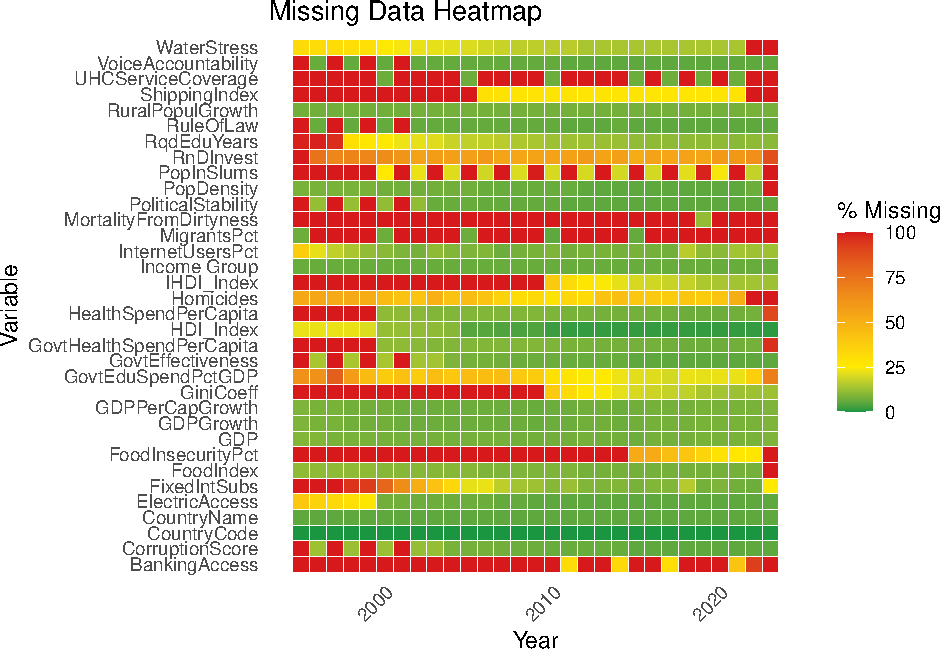
\includegraphics[keepaspectratio]{Exploratory-Data-Analysis_files/figure-latex/MissingnessGrid-1.pdf}}

\begin{Shaded}
\begin{Highlighting}[]
\NormalTok{FirstCutData }\SpecialCharTok{\%\textgreater{}\%}
  \FunctionTok{summarise}\NormalTok{(}\FunctionTok{across}\NormalTok{(}\FunctionTok{everything}\NormalTok{(), }\SpecialCharTok{\textasciitilde{}} \FunctionTok{mean}\NormalTok{(}\FunctionTok{is.na}\NormalTok{(.)) }\SpecialCharTok{*} \DecValTok{100}\NormalTok{)) }\SpecialCharTok{\%\textgreater{}\%}
  \FunctionTok{pivot\_longer}\NormalTok{(}\AttributeTok{cols =} \FunctionTok{everything}\NormalTok{(), }\AttributeTok{names\_to =} \StringTok{"Variable"}\NormalTok{, }\AttributeTok{values\_to =} \StringTok{"MissingPct"}\NormalTok{) }\SpecialCharTok{\%\textgreater{}\%}
  \FunctionTok{ggplot}\NormalTok{(}\FunctionTok{aes}\NormalTok{(}\AttributeTok{x =} \FunctionTok{reorder}\NormalTok{(Variable, MissingPct), }\AttributeTok{y =}\NormalTok{ MissingPct, }\AttributeTok{fill =}\NormalTok{ MissingPct)) }\SpecialCharTok{+}
  \FunctionTok{geom\_col}\NormalTok{() }\SpecialCharTok{+}
  \FunctionTok{coord\_flip}\NormalTok{() }\SpecialCharTok{+}
  \FunctionTok{scale\_fill\_gradientn}\NormalTok{(}
    \AttributeTok{colors =}\NormalTok{ stoplight,}
    \AttributeTok{limits =} \FunctionTok{c}\NormalTok{(}\DecValTok{0}\NormalTok{, }\DecValTok{100}\NormalTok{),}
    \AttributeTok{breaks =} \FunctionTok{c}\NormalTok{(}\DecValTok{0}\NormalTok{, }\DecValTok{25}\NormalTok{, }\DecValTok{50}\NormalTok{, }\DecValTok{75}\NormalTok{, }\DecValTok{100}\NormalTok{),  }\CommentTok{\# include 0 and 100}
    \AttributeTok{labels =} \FunctionTok{c}\NormalTok{(}\StringTok{"0"}\NormalTok{, }\StringTok{"25"}\NormalTok{, }\StringTok{"50"}\NormalTok{, }\StringTok{"75"}\NormalTok{, }\StringTok{"100"}\NormalTok{),}
    \AttributeTok{name =} \StringTok{"\% Missing"}
\NormalTok{  ) }\SpecialCharTok{+}
  \FunctionTok{labs}\NormalTok{(}
    \AttributeTok{title =} \StringTok{"Overall Sparseness by Variable"}\NormalTok{,}
    \AttributeTok{x =} \StringTok{"Variable"}\NormalTok{,}
    \AttributeTok{y =} \StringTok{"\% Missing"}
\NormalTok{  ) }\SpecialCharTok{+}
  \FunctionTok{theme\_minimal}\NormalTok{()}
\end{Highlighting}
\end{Shaded}

\pandocbounded{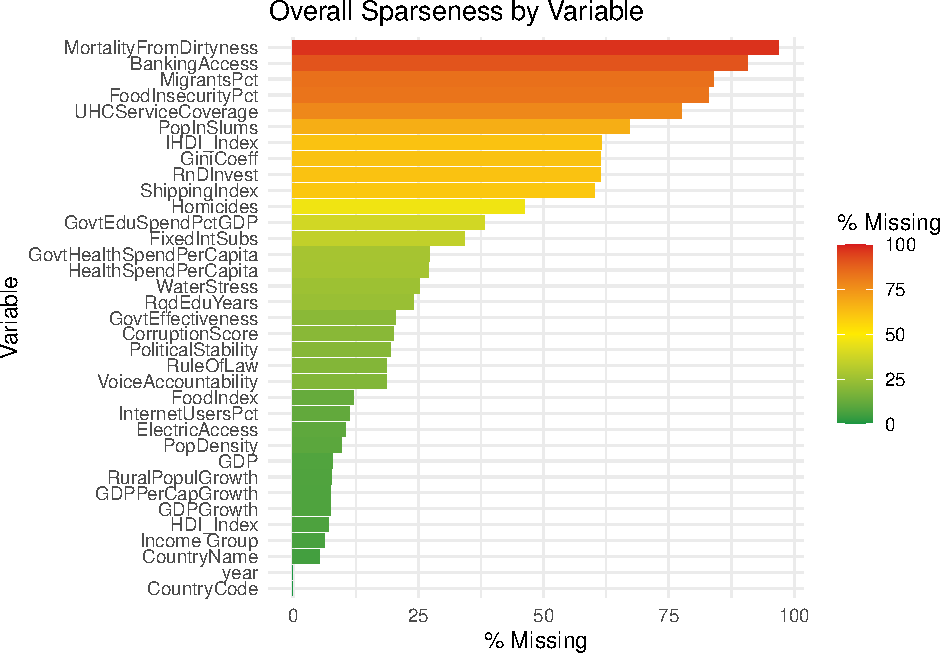
\includegraphics[keepaspectratio]{Exploratory-Data-Analysis_files/figure-latex/MissingnessSummary-1.pdf}}

\begin{Shaded}
\begin{Highlighting}[]
\NormalTok{FirstCutData }\SpecialCharTok{\%\textgreater{}\%}
  \FunctionTok{group\_by}\NormalTok{(year) }\SpecialCharTok{\%\textgreater{}\%}
  \FunctionTok{summarise}\NormalTok{(}\FunctionTok{across}\NormalTok{(}\FunctionTok{everything}\NormalTok{(), }\SpecialCharTok{\textasciitilde{}} \FunctionTok{mean}\NormalTok{(}\FunctionTok{is.na}\NormalTok{(.)) }\SpecialCharTok{*} \DecValTok{100}\NormalTok{)) }\SpecialCharTok{\%\textgreater{}\%}
  \FunctionTok{pivot\_longer}\NormalTok{(}\SpecialCharTok{{-}}\NormalTok{year, }\AttributeTok{names\_to =} \StringTok{"variable"}\NormalTok{, }\AttributeTok{values\_to =} \StringTok{"pct\_missing"}\NormalTok{) }\SpecialCharTok{\%\textgreater{}\%}
  \FunctionTok{group\_by}\NormalTok{(year) }\SpecialCharTok{\%\textgreater{}\%}
  \FunctionTok{summarise}\NormalTok{(}\AttributeTok{pct\_missing =} \FunctionTok{mean}\NormalTok{(pct\_missing)) }\SpecialCharTok{\%\textgreater{}\%}
  \FunctionTok{arrange}\NormalTok{(year) }\SpecialCharTok{\%\textgreater{}\%}
  \FunctionTok{ggplot}\NormalTok{(}\FunctionTok{aes}\NormalTok{(}\AttributeTok{y =} \FunctionTok{factor}\NormalTok{(year), }\AttributeTok{x =}\NormalTok{ pct\_missing, }\AttributeTok{fill =}\NormalTok{ pct\_missing)) }\SpecialCharTok{+}
  \FunctionTok{geom\_col}\NormalTok{() }\SpecialCharTok{+}
  \FunctionTok{scale\_fill\_gradientn}\NormalTok{(}
    \AttributeTok{colors =}\NormalTok{ stoplight,}
    \AttributeTok{values =} \FunctionTok{rescale}\NormalTok{(}\FunctionTok{c}\NormalTok{(}\DecValTok{0}\NormalTok{, }\DecValTok{50}\NormalTok{, }\DecValTok{100}\NormalTok{)),}
    \AttributeTok{name =} \StringTok{"\% Missing"}\NormalTok{,}
    \AttributeTok{limits =} \FunctionTok{c}\NormalTok{(}\DecValTok{0}\NormalTok{, }\DecValTok{100}\NormalTok{),}
    \AttributeTok{breaks =} \FunctionTok{c}\NormalTok{(}\DecValTok{0}\NormalTok{, }\DecValTok{50}\NormalTok{, }\DecValTok{100}\NormalTok{),}
    \AttributeTok{labels =} \FunctionTok{c}\NormalTok{(}\StringTok{"0"}\NormalTok{, }\StringTok{"50"}\NormalTok{, }\StringTok{"100"}\NormalTok{)}
\NormalTok{  ) }\SpecialCharTok{+}
  \FunctionTok{labs}\NormalTok{(}
    \AttributeTok{y =} \StringTok{"Year"}\NormalTok{,}
    \AttributeTok{x =} \StringTok{"\% Missing (All Variables)"}\NormalTok{,}
    \AttributeTok{title =} \StringTok{"Data Sparseness by Year"}
\NormalTok{  ) }\SpecialCharTok{+}
  \FunctionTok{theme\_minimal}\NormalTok{() }\SpecialCharTok{+}
  \FunctionTok{theme}\NormalTok{(}
    \AttributeTok{axis.text.y =} \FunctionTok{element\_text}\NormalTok{(}\AttributeTok{size =} \DecValTok{8}\NormalTok{),}
    \AttributeTok{legend.position =} \StringTok{"right"}
\NormalTok{  )}
\end{Highlighting}
\end{Shaded}

\pandocbounded{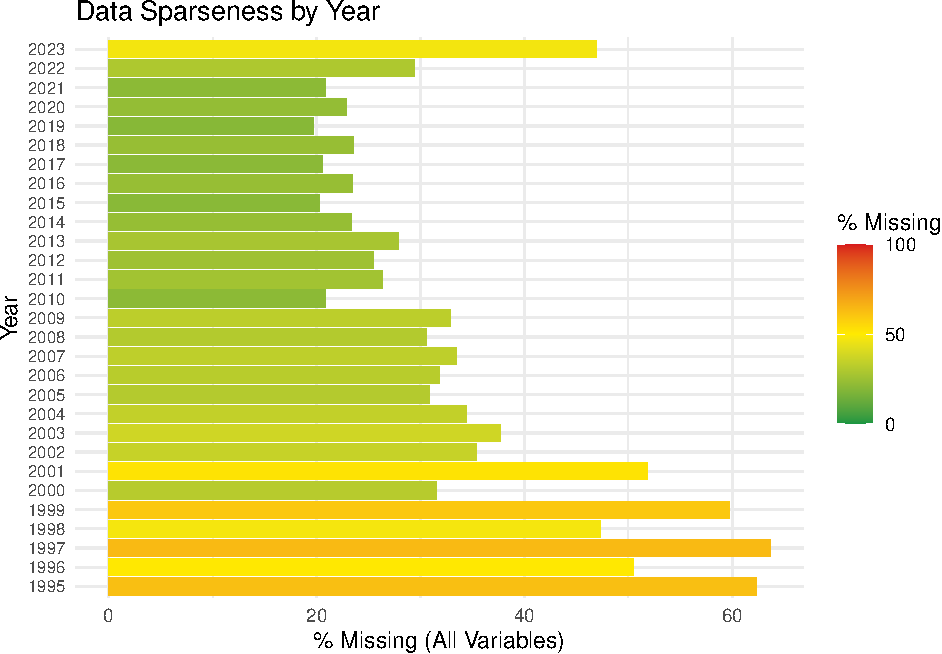
\includegraphics[keepaspectratio]{Exploratory-Data-Analysis_files/figure-latex/MissingnessSummary-2.pdf}}

\begin{Shaded}
\begin{Highlighting}[]
\CommentTok{\# Time series analysis}

\CommentTok{\# Overall averages}





\CommentTok{\# Prep data}
\NormalTok{FirstCut\_Yearly\_Avg }\OtherTok{\textless{}{-}}\NormalTok{ FirstCutData }\SpecialCharTok{\%\textgreater{}\%}
  \FunctionTok{group\_by}\NormalTok{(year) }\SpecialCharTok{\%\textgreater{}\%}
  \FunctionTok{summarize}\NormalTok{(}
    \AttributeTok{InternetUsers =} \FunctionTok{mean}\NormalTok{(InternetUsersPct, }\AttributeTok{na.rm =} \ConstantTok{TRUE}\NormalTok{)}\SpecialCharTok{/}\DecValTok{100}\NormalTok{,}
    \AttributeTok{HDI =} \FunctionTok{mean}\NormalTok{(HDI\_Index, }\AttributeTok{na.rm =} \ConstantTok{TRUE}\NormalTok{),}
    \AttributeTok{.groups =} \StringTok{"drop"}
\NormalTok{  ) }\SpecialCharTok{\%\textgreater{}\%}
  \FunctionTok{mutate}\NormalTok{(}
    \AttributeTok{HDI\_scaled =}\NormalTok{ (HDI }\SpecialCharTok{{-}} \FloatTok{0.6}\NormalTok{) }\SpecialCharTok{/} \FloatTok{0.4}  \CommentTok{\# rescale onto same scale as inernet users}
\NormalTok{  )}

\CommentTok{\# Plot with dual axes}
\FunctionTok{ggplot}\NormalTok{(FirstCut\_Yearly\_Avg, }\FunctionTok{aes}\NormalTok{(}\AttributeTok{x =}\NormalTok{ year)) }\SpecialCharTok{+}
  \FunctionTok{geom\_line}\NormalTok{(}\FunctionTok{aes}\NormalTok{(}\AttributeTok{y =}\NormalTok{ InternetUsers, }\AttributeTok{color =} \StringTok{"Internet Users (\%)"}\NormalTok{), }\AttributeTok{size =} \FloatTok{1.2}\NormalTok{) }\SpecialCharTok{+}
  \FunctionTok{geom\_line}\NormalTok{(}\FunctionTok{aes}\NormalTok{(}\AttributeTok{y =}\NormalTok{ HDI\_scaled, }\AttributeTok{color =} \StringTok{"HDI"}\NormalTok{), }\AttributeTok{size =} \FloatTok{1.2}\NormalTok{) }\SpecialCharTok{+}
  \FunctionTok{scale\_x\_continuous}\NormalTok{(}\AttributeTok{breaks =} \FunctionTok{seq}\NormalTok{(}\DecValTok{1995}\NormalTok{, }\DecValTok{2025}\NormalTok{, }\AttributeTok{by =} \DecValTok{2}\NormalTok{))}\SpecialCharTok{+}
  \FunctionTok{scale\_y\_continuous}\NormalTok{(}
    \AttributeTok{name =} \StringTok{"Internet Users (\%)"}\NormalTok{,}
    \AttributeTok{labels =}\NormalTok{ scales}\SpecialCharTok{::}\NormalTok{percent,}
    \AttributeTok{limits =} \FunctionTok{c}\NormalTok{(}\DecValTok{0}\NormalTok{, }\FloatTok{0.75}\NormalTok{),  }\CommentTok{\# force axis to run from 0\% to 75\%}
    \AttributeTok{sec.axis =} \FunctionTok{sec\_axis}\NormalTok{(}\SpecialCharTok{\textasciitilde{}}\NormalTok{ . }\SpecialCharTok{*} \FloatTok{0.4} \SpecialCharTok{+} \FloatTok{0.6}\NormalTok{, }\AttributeTok{name =} \StringTok{"HDI"}\NormalTok{) }\CommentTok{\# label axis correctly }
\NormalTok{  ) }\SpecialCharTok{+}
  \FunctionTok{scale\_color\_manual}\NormalTok{(}\AttributeTok{values =} \FunctionTok{c}\NormalTok{(}\StringTok{"Internet Users (\%)"} \OtherTok{=} \StringTok{"\#00BFC4"}\NormalTok{, }\StringTok{"HDI"} \OtherTok{=} \StringTok{"\#F8766D"}\NormalTok{)) }\SpecialCharTok{+}
  \FunctionTok{labs}\NormalTok{(}
    \AttributeTok{title =} \StringTok{"Global Average Internet Use and HDI Over Time"}\NormalTok{,}
    \AttributeTok{x =} \StringTok{"Year"}\NormalTok{,}
    \AttributeTok{color =} \StringTok{""}
\NormalTok{  ) }\SpecialCharTok{+}
  \FunctionTok{theme\_minimal}\NormalTok{(}\AttributeTok{base\_size =} \DecValTok{14}\NormalTok{) }\SpecialCharTok{+}
  \FunctionTok{theme}\NormalTok{(}
    \AttributeTok{legend.position =} \StringTok{"bottom"}\NormalTok{,}
    \AttributeTok{plot.title =} \FunctionTok{element\_text}\NormalTok{(}\AttributeTok{face =} \StringTok{"bold"}\NormalTok{, }\AttributeTok{hjust =} \FloatTok{0.5}\NormalTok{)}
\NormalTok{  )}
\end{Highlighting}
\end{Shaded}

\begin{verbatim}
## Warning: Using `size` aesthetic for lines was deprecated in ggplot2 3.4.0.
## i Please use `linewidth` instead.
## This warning is displayed once every 8 hours.
## Call `lifecycle::last_lifecycle_warnings()` to see where this warning was
## generated.
\end{verbatim}

\pandocbounded{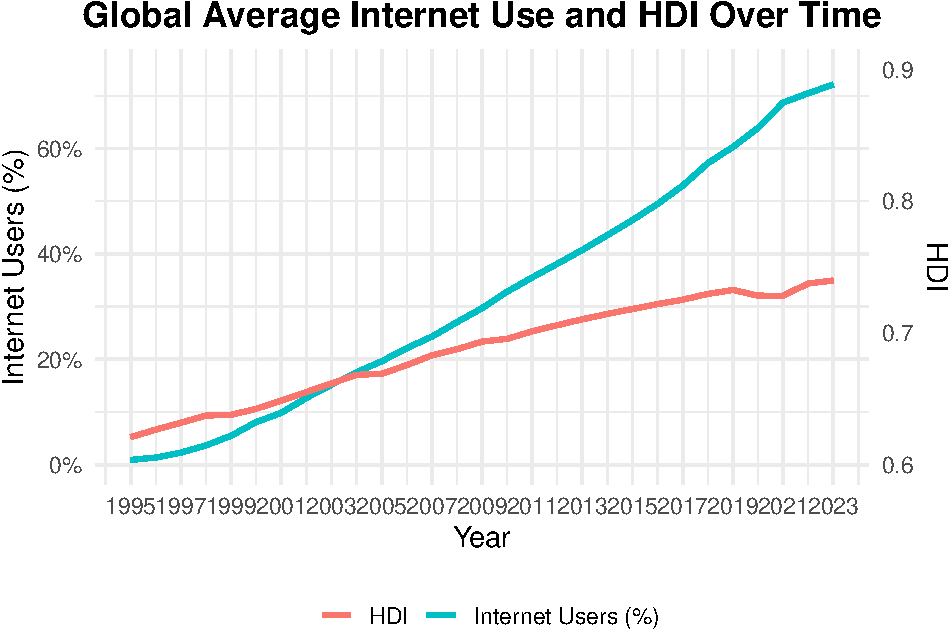
\includegraphics[keepaspectratio]{Exploratory-Data-Analysis_files/figure-latex/TimeSeries-1.pdf}}

\begin{Shaded}
\begin{Highlighting}[]
\CommentTok{\# Group and summarize}
\NormalTok{FirstCut\_Yearly\_Income\_Avg }\OtherTok{\textless{}{-}}\NormalTok{ FirstCutDataFiltered }\SpecialCharTok{\%\textgreater{}\%}
  \FunctionTok{group\_by}\NormalTok{(year, }\StringTok{\textasciigrave{}}\AttributeTok{Income Group}\StringTok{\textasciigrave{}}\NormalTok{) }\SpecialCharTok{\%\textgreater{}\%}
  \FunctionTok{summarize}\NormalTok{(}
    \StringTok{\textasciigrave{}}\AttributeTok{Internet Users (\%)}\StringTok{\textasciigrave{}} \OtherTok{=} \FunctionTok{mean}\NormalTok{(InternetUsersPct, }\AttributeTok{na.rm =} \ConstantTok{TRUE}\NormalTok{)}\SpecialCharTok{/}\DecValTok{100}\NormalTok{,}
    \StringTok{\textasciigrave{}}\AttributeTok{HDI}\StringTok{\textasciigrave{}} \OtherTok{=} \FunctionTok{mean}\NormalTok{(HDI\_Index, }\AttributeTok{na.rm =} \ConstantTok{TRUE}\NormalTok{),}
    \AttributeTok{.groups =} \StringTok{"drop"}
\NormalTok{  )}

\CommentTok{\# Pivot to long format}
\NormalTok{FirstCut\_Yearly\_Income\_Avg\_Long }\OtherTok{\textless{}{-}}\NormalTok{ FirstCut\_Yearly\_Income\_Avg }\SpecialCharTok{\%\textgreater{}\%}
  \FunctionTok{pivot\_longer}\NormalTok{(}\AttributeTok{cols =} \FunctionTok{c}\NormalTok{(}\StringTok{\textasciigrave{}}\AttributeTok{Internet Users (\%)}\StringTok{\textasciigrave{}}\NormalTok{, }\StringTok{\textasciigrave{}}\AttributeTok{HDI}\StringTok{\textasciigrave{}}\NormalTok{),}
               \AttributeTok{names\_to =} \StringTok{"Metric"}\NormalTok{, }\AttributeTok{values\_to =} \StringTok{"Value"}\NormalTok{)}

\CommentTok{\# Plot {-} facet by Income Group (columns) and Metric (rows), color by Metric}
\FunctionTok{ggplot}\NormalTok{(FirstCut\_Yearly\_Income\_Avg\_Long,}
       \FunctionTok{aes}\NormalTok{(}\AttributeTok{x =}\NormalTok{ year, }\AttributeTok{y =}\NormalTok{ Value, }\AttributeTok{color =}\NormalTok{ Metric)) }\SpecialCharTok{+}
  \FunctionTok{geom\_line}\NormalTok{(}\AttributeTok{size =} \FloatTok{1.2}\NormalTok{) }\SpecialCharTok{+}
  \FunctionTok{facet\_grid}\NormalTok{(Metric }\SpecialCharTok{\textasciitilde{}} \StringTok{\textasciigrave{}}\AttributeTok{Income Group}\StringTok{\textasciigrave{}}\NormalTok{, }\AttributeTok{scales =} \StringTok{"free\_y"}\NormalTok{) }\SpecialCharTok{+}
  \FunctionTok{scale\_color\_manual}\NormalTok{(}\AttributeTok{values =} \FunctionTok{c}\NormalTok{(}
    \StringTok{"HDI"} \OtherTok{=} \StringTok{"\#F8766D"}\NormalTok{,}
    \StringTok{"Internet Users (\%)"} \OtherTok{=} \StringTok{"\#00BFC4"}
\NormalTok{  )) }\SpecialCharTok{+}
  \FunctionTok{labs}\NormalTok{(}
    \AttributeTok{title =} \StringTok{"Internet Access and HDI Over Time by Income Group"}\NormalTok{,}
    \AttributeTok{x =} \StringTok{"Year"}\NormalTok{,}
    \AttributeTok{y =} \StringTok{"Average Value"}\NormalTok{,}
    \AttributeTok{color =} \StringTok{""}
\NormalTok{  ) }\SpecialCharTok{+}
  \FunctionTok{theme\_minimal}\NormalTok{(}\AttributeTok{base\_size =} \DecValTok{14}\NormalTok{) }\SpecialCharTok{+}
  \FunctionTok{theme}\NormalTok{(}
    \AttributeTok{legend.position =} \StringTok{"bottom"}\NormalTok{,}
    \AttributeTok{strip.text =} \FunctionTok{element\_text}\NormalTok{(}\AttributeTok{face =} \StringTok{"bold"}\NormalTok{, }\AttributeTok{size =} \DecValTok{12}\NormalTok{),}
    \AttributeTok{plot.title =} \FunctionTok{element\_text}\NormalTok{(}\AttributeTok{face =} \StringTok{"bold"}\NormalTok{, }\AttributeTok{hjust =} \FloatTok{0.5}\NormalTok{),}
    \AttributeTok{axis.text.x =} \FunctionTok{element\_text}\NormalTok{(}\AttributeTok{size =} \DecValTok{9}\NormalTok{, }\AttributeTok{angle =} \DecValTok{45}\NormalTok{, }\AttributeTok{hjust =} \DecValTok{1}\NormalTok{)  }\CommentTok{\# 👈 the fix}
\NormalTok{  )}
\end{Highlighting}
\end{Shaded}

\pandocbounded{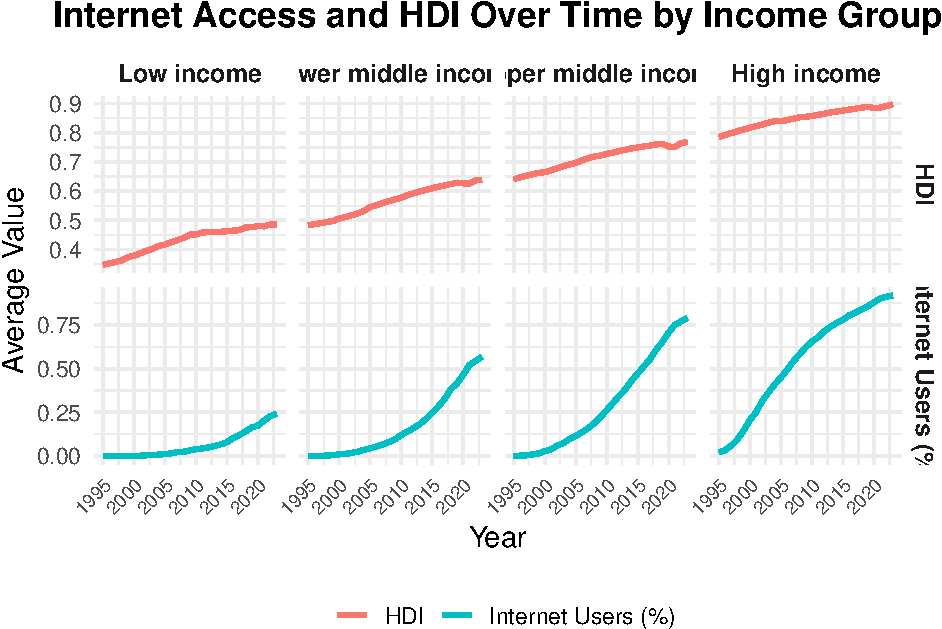
\includegraphics[keepaspectratio]{Exploratory-Data-Analysis_files/figure-latex/TimeSeries-2.pdf}}

\begin{Shaded}
\begin{Highlighting}[]
\CommentTok{\# Filter to Low Income only}
\NormalTok{LowIncome\_Yearly\_Avg }\OtherTok{\textless{}{-}}\NormalTok{ FirstCutDataFiltered }\SpecialCharTok{\%\textgreater{}\%}
  \FunctionTok{filter}\NormalTok{(}\StringTok{\textasciigrave{}}\AttributeTok{Income Group}\StringTok{\textasciigrave{}} \SpecialCharTok{==} \StringTok{"Low income"}\NormalTok{) }\SpecialCharTok{\%\textgreater{}\%}
  \FunctionTok{group\_by}\NormalTok{(year) }\SpecialCharTok{\%\textgreater{}\%}
  \FunctionTok{summarize}\NormalTok{(}
    \StringTok{\textasciigrave{}}\AttributeTok{Internet Users (\%)}\StringTok{\textasciigrave{}} \OtherTok{=} \FunctionTok{mean}\NormalTok{(InternetUsersPct, }\AttributeTok{na.rm =} \ConstantTok{TRUE}\NormalTok{)}\SpecialCharTok{/}\DecValTok{100}\NormalTok{,}
    \StringTok{\textasciigrave{}}\AttributeTok{HDI}\StringTok{\textasciigrave{}} \OtherTok{=} \FunctionTok{mean}\NormalTok{(HDI\_Index, }\AttributeTok{na.rm =} \ConstantTok{TRUE}\NormalTok{),}
    \AttributeTok{.groups =} \StringTok{"drop"}
\NormalTok{  ) }\SpecialCharTok{\%\textgreater{}\%}
  \FunctionTok{pivot\_longer}\NormalTok{(}\AttributeTok{cols =} \FunctionTok{c}\NormalTok{(}\StringTok{\textasciigrave{}}\AttributeTok{Internet Users (\%)}\StringTok{\textasciigrave{}}\NormalTok{, }\StringTok{\textasciigrave{}}\AttributeTok{HDI}\StringTok{\textasciigrave{}}\NormalTok{),}
               \AttributeTok{names\_to =} \StringTok{"Metric"}\NormalTok{, }\AttributeTok{values\_to =} \StringTok{"Value"}\NormalTok{)}

\CommentTok{\# Plot with HDI and Internet Users (\%) stacked vertically}
\FunctionTok{ggplot}\NormalTok{(LowIncome\_Yearly\_Avg, }\FunctionTok{aes}\NormalTok{(}\AttributeTok{x =}\NormalTok{ year, }\AttributeTok{y =}\NormalTok{ Value, }\AttributeTok{color =}\NormalTok{ Metric)) }\SpecialCharTok{+}
  \FunctionTok{geom\_line}\NormalTok{(}\AttributeTok{size =} \FloatTok{1.2}\NormalTok{) }\SpecialCharTok{+}
  \FunctionTok{facet\_wrap}\NormalTok{(}\SpecialCharTok{\textasciitilde{}}\NormalTok{ Metric, }\AttributeTok{ncol =} \DecValTok{1}\NormalTok{, }\AttributeTok{scales =} \StringTok{"free\_y"}\NormalTok{) }\SpecialCharTok{+}
  \FunctionTok{scale\_color\_manual}\NormalTok{(}\AttributeTok{values =} \FunctionTok{c}\NormalTok{(}
    \StringTok{"HDI"} \OtherTok{=} \StringTok{"\#F8766D"}\NormalTok{,}
    \StringTok{"Internet Users (\%)"} \OtherTok{=} \StringTok{"\#00BFC4"}
\NormalTok{  )) }\SpecialCharTok{+}
  \FunctionTok{scale\_x\_continuous}\NormalTok{(}\AttributeTok{breaks =} \FunctionTok{seq}\NormalTok{(}\DecValTok{1995}\NormalTok{, }\DecValTok{2025}\NormalTok{, }\DecValTok{2}\NormalTok{)) }\SpecialCharTok{+}
  \FunctionTok{labs}\NormalTok{(}
    \AttributeTok{title =} \StringTok{"Time Trends of Internet Access and HDI (Low Income Countries)"}\NormalTok{,}
    \AttributeTok{x =} \StringTok{"Year"}\NormalTok{,}
    \AttributeTok{y =} \StringTok{"Average Value"}\NormalTok{,}
    \AttributeTok{color =} \StringTok{""}
\NormalTok{  ) }\SpecialCharTok{+}
  \FunctionTok{theme\_minimal}\NormalTok{(}\AttributeTok{base\_size =} \DecValTok{14}\NormalTok{) }\SpecialCharTok{+}
  \FunctionTok{theme}\NormalTok{(}
    \AttributeTok{legend.position =} \StringTok{"bottom"}\NormalTok{,}
    \AttributeTok{strip.text =} \FunctionTok{element\_text}\NormalTok{(}\AttributeTok{face =} \StringTok{"bold"}\NormalTok{, }\AttributeTok{size =} \DecValTok{12}\NormalTok{),}
    \AttributeTok{plot.title =} \FunctionTok{element\_text}\NormalTok{(}\AttributeTok{face =} \StringTok{"bold"}\NormalTok{, }\AttributeTok{hjust =} \FloatTok{0.5}\NormalTok{),}
    \AttributeTok{axis.text.x =} \FunctionTok{element\_text}\NormalTok{(}\AttributeTok{size =} \DecValTok{9}\NormalTok{, }\AttributeTok{angle =} \DecValTok{45}\NormalTok{, }\AttributeTok{hjust =} \DecValTok{1}\NormalTok{)}
\NormalTok{  )}
\end{Highlighting}
\end{Shaded}

\pandocbounded{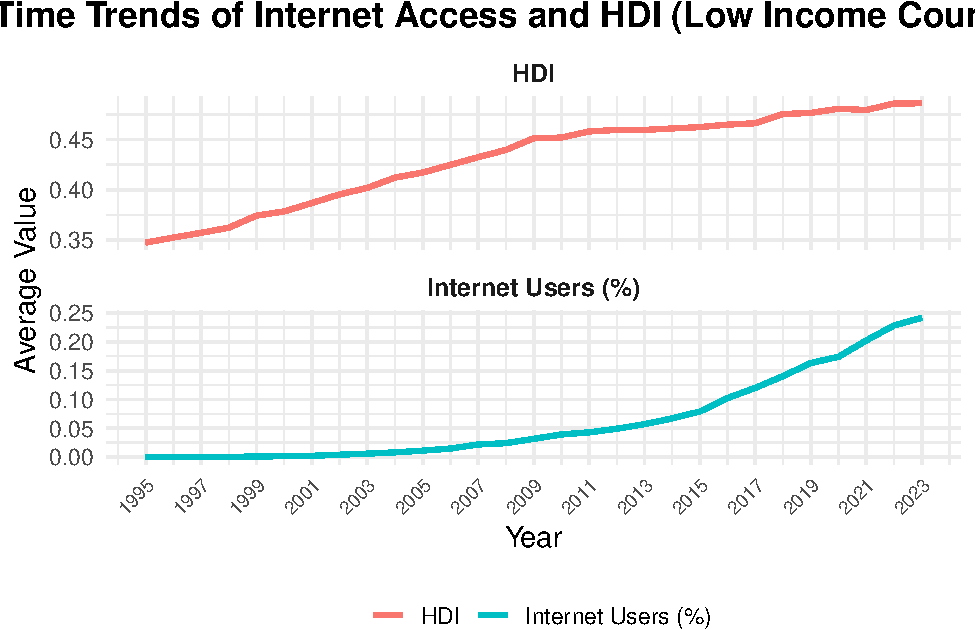
\includegraphics[keepaspectratio]{Exploratory-Data-Analysis_files/figure-latex/TimeSeries-3.pdf}}

\begin{Shaded}
\begin{Highlighting}[]
\CommentTok{\# Create groupings}
\NormalTok{LowIncome\_Yearly\_Avg }\OtherTok{\textless{}{-}}\NormalTok{ FirstCutDataFiltered }\SpecialCharTok{\%\textgreater{}\%}
  \FunctionTok{filter}\NormalTok{(}\StringTok{\textasciigrave{}}\AttributeTok{Income Group}\StringTok{\textasciigrave{}} \SpecialCharTok{==} \StringTok{"Low income"}\NormalTok{) }\SpecialCharTok{\%\textgreater{}\%}
  \FunctionTok{group\_by}\NormalTok{(year) }\SpecialCharTok{\%\textgreater{}\%}
  \FunctionTok{summarize}\NormalTok{(}
    \StringTok{\textasciigrave{}}\AttributeTok{Internet Users (\%)}\StringTok{\textasciigrave{}} \OtherTok{=} \FunctionTok{mean}\NormalTok{(InternetUsersPct, }\AttributeTok{na.rm =} \ConstantTok{TRUE}\NormalTok{)}\SpecialCharTok{/}\DecValTok{100}\NormalTok{,}
    \StringTok{\textasciigrave{}}\AttributeTok{HDI}\StringTok{\textasciigrave{}} \OtherTok{=} \FunctionTok{mean}\NormalTok{(HDI\_Index, }\AttributeTok{na.rm =} \ConstantTok{TRUE}\NormalTok{),}
    \StringTok{\textasciigrave{}}\AttributeTok{IHDI}\StringTok{\textasciigrave{}} \OtherTok{=} \FunctionTok{mean}\NormalTok{(IHDI\_Index, }\AttributeTok{na.rm =} \ConstantTok{TRUE}\NormalTok{),}
    \AttributeTok{.groups =} \StringTok{"drop"}
\NormalTok{  ) }\SpecialCharTok{\%\textgreater{}\%}
  \FunctionTok{pivot\_longer}\NormalTok{(}\AttributeTok{cols =} \FunctionTok{c}\NormalTok{(}\StringTok{\textasciigrave{}}\AttributeTok{Internet Users (\%)}\StringTok{\textasciigrave{}}\NormalTok{, }\StringTok{\textasciigrave{}}\AttributeTok{HDI}\StringTok{\textasciigrave{}}\NormalTok{, }\StringTok{\textasciigrave{}}\AttributeTok{IHDI}\StringTok{\textasciigrave{}}\NormalTok{),}
               \AttributeTok{names\_to =} \StringTok{"Metric"}\NormalTok{, }\AttributeTok{values\_to =} \StringTok{"Value"}\NormalTok{) }\SpecialCharTok{\%\textgreater{}\%}
  \FunctionTok{mutate}\NormalTok{(}
    \AttributeTok{MetricGroup =} \FunctionTok{ifelse}\NormalTok{(Metric }\SpecialCharTok{\%in\%} \FunctionTok{c}\NormalTok{(}\StringTok{"HDI"}\NormalTok{, }\StringTok{"IHDI"}\NormalTok{),}
                         \StringTok{"Wellbeing Index"}\NormalTok{,}
                         \StringTok{"Internet Access"}\NormalTok{)}
\NormalTok{  )}

\CommentTok{\# Reorder facet levels so Wellbeing is on top}
\NormalTok{LowIncome\_Yearly\_Avg}\SpecialCharTok{$}\NormalTok{MetricGroup }\OtherTok{\textless{}{-}} \FunctionTok{factor}\NormalTok{(}
\NormalTok{  LowIncome\_Yearly\_Avg}\SpecialCharTok{$}\NormalTok{MetricGroup,}
  \AttributeTok{levels =} \FunctionTok{c}\NormalTok{(}\StringTok{"Wellbeing Index"}\NormalTok{, }\StringTok{"Internet Access"}\NormalTok{)}
\NormalTok{)}

\CommentTok{\# Plot}
\FunctionTok{ggplot}\NormalTok{(LowIncome\_Yearly\_Avg, }\FunctionTok{aes}\NormalTok{(}\AttributeTok{x =}\NormalTok{ year, }\AttributeTok{y =}\NormalTok{ Value, }\AttributeTok{color =}\NormalTok{ Metric)) }\SpecialCharTok{+}
  \FunctionTok{geom\_line}\NormalTok{(}\AttributeTok{size =} \FloatTok{1.2}\NormalTok{) }\SpecialCharTok{+}
  \FunctionTok{facet\_wrap}\NormalTok{(}\SpecialCharTok{\textasciitilde{}}\NormalTok{ MetricGroup, }\AttributeTok{ncol =} \DecValTok{1}\NormalTok{, }\AttributeTok{scales =} \StringTok{"free\_y"}\NormalTok{) }\SpecialCharTok{+}
  \FunctionTok{scale\_color\_manual}\NormalTok{(}\AttributeTok{values =} \FunctionTok{c}\NormalTok{(}
    \StringTok{"HDI"} \OtherTok{=} \StringTok{"\#F8766D"}\NormalTok{,}
    \StringTok{"IHDI"} \OtherTok{=} \StringTok{"\#D89000"}\NormalTok{,}
    \StringTok{"Internet Users (\%)"} \OtherTok{=} \StringTok{"\#00BFC4"}
\NormalTok{  )) }\SpecialCharTok{+}
  \FunctionTok{scale\_x\_continuous}\NormalTok{(}\AttributeTok{breaks =} \FunctionTok{seq}\NormalTok{(}\DecValTok{1995}\NormalTok{, }\DecValTok{2025}\NormalTok{, }\DecValTok{2}\NormalTok{)) }\SpecialCharTok{+}
  \FunctionTok{labs}\NormalTok{(}
    \AttributeTok{title =} \StringTok{"HDI, IHDI, and Internet Access Over Time (Low Income Countries)"}\NormalTok{,}
    \AttributeTok{x =} \StringTok{"Year"}\NormalTok{,}
    \AttributeTok{y =} \StringTok{"Average Value"}\NormalTok{,}
    \AttributeTok{color =} \StringTok{""}
\NormalTok{  ) }\SpecialCharTok{+}
  \FunctionTok{theme\_minimal}\NormalTok{(}\AttributeTok{base\_size =} \DecValTok{14}\NormalTok{) }\SpecialCharTok{+}
  \FunctionTok{theme}\NormalTok{(}
    \AttributeTok{legend.position =} \StringTok{"bottom"}\NormalTok{,}
    \AttributeTok{strip.text =} \FunctionTok{element\_text}\NormalTok{(}\AttributeTok{face =} \StringTok{"bold"}\NormalTok{, }\AttributeTok{size =} \DecValTok{12}\NormalTok{),}
    \AttributeTok{plot.title =} \FunctionTok{element\_text}\NormalTok{(}\AttributeTok{face =} \StringTok{"bold"}\NormalTok{, }\AttributeTok{hjust =} \FloatTok{0.5}\NormalTok{),}
    \AttributeTok{axis.text.x =} \FunctionTok{element\_text}\NormalTok{(}\AttributeTok{size =} \DecValTok{9}\NormalTok{, }\AttributeTok{angle =} \DecValTok{45}\NormalTok{, }\AttributeTok{hjust =} \DecValTok{1}\NormalTok{)}
\NormalTok{  )}
\end{Highlighting}
\end{Shaded}

\begin{verbatim}
## Warning: Removed 15 rows containing missing values or values outside the scale range
## (`geom_line()`).
\end{verbatim}

\pandocbounded{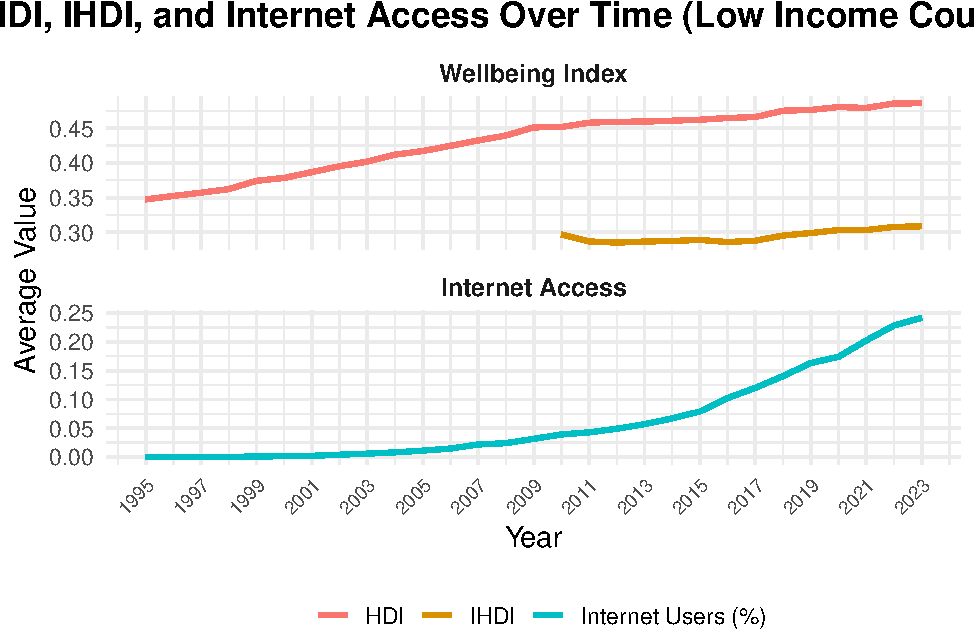
\includegraphics[keepaspectratio]{Exploratory-Data-Analysis_files/figure-latex/TimeSeries-4.pdf}}

\end{document}
